\section{Gjennomføring med måleresultater}
I denne seksjonen presenteres måleresultater for alle kretsene som er koblet opp i forsøket. For hver krets presenteres en kort beskrivelse av fremgangsmåten for oppkobling og måling, oscilloskopbilde, etterfulgt av en grafisk fremstilling av målingen på oscilloskopet for å enklere fremstille verdier på akser. I tillegg kommenteres resultatene for hver krets, hvor det gir en kort vurdering av om resultatet er som forventet og om det er noen avvik fra det teoretiske resultatet. Diskusjoner knyttet til resultatene vil bli presentert i diskusjonsseksjonen senere i rapporten.

\subsection{Krets 1 -- enveis klippekrets}
Fremgangsmåten for å koble opp denne kretsen blir å bruke komponentene i kretsen i figur~\ref{fig:krets1} og koble dem opp på et breadboard. Signalgeneratoren stilles inn på en sinusformet spenning med toppverdi $10\mathrm{V}$ og frekvens $50\mathrm{Hz}$. Deretter bruker vi en motstand på $180\Omega$ i serie med dioden. For å måle klippekretsspenningen, bruker vi oscilloskopet. En kanal kobles til inngangsspenningen, og en annen kanal kobles over dioden. Resultatene er presentert i figurene under.

\vspace{3em}

\begin{figure}[H]
    \centering
    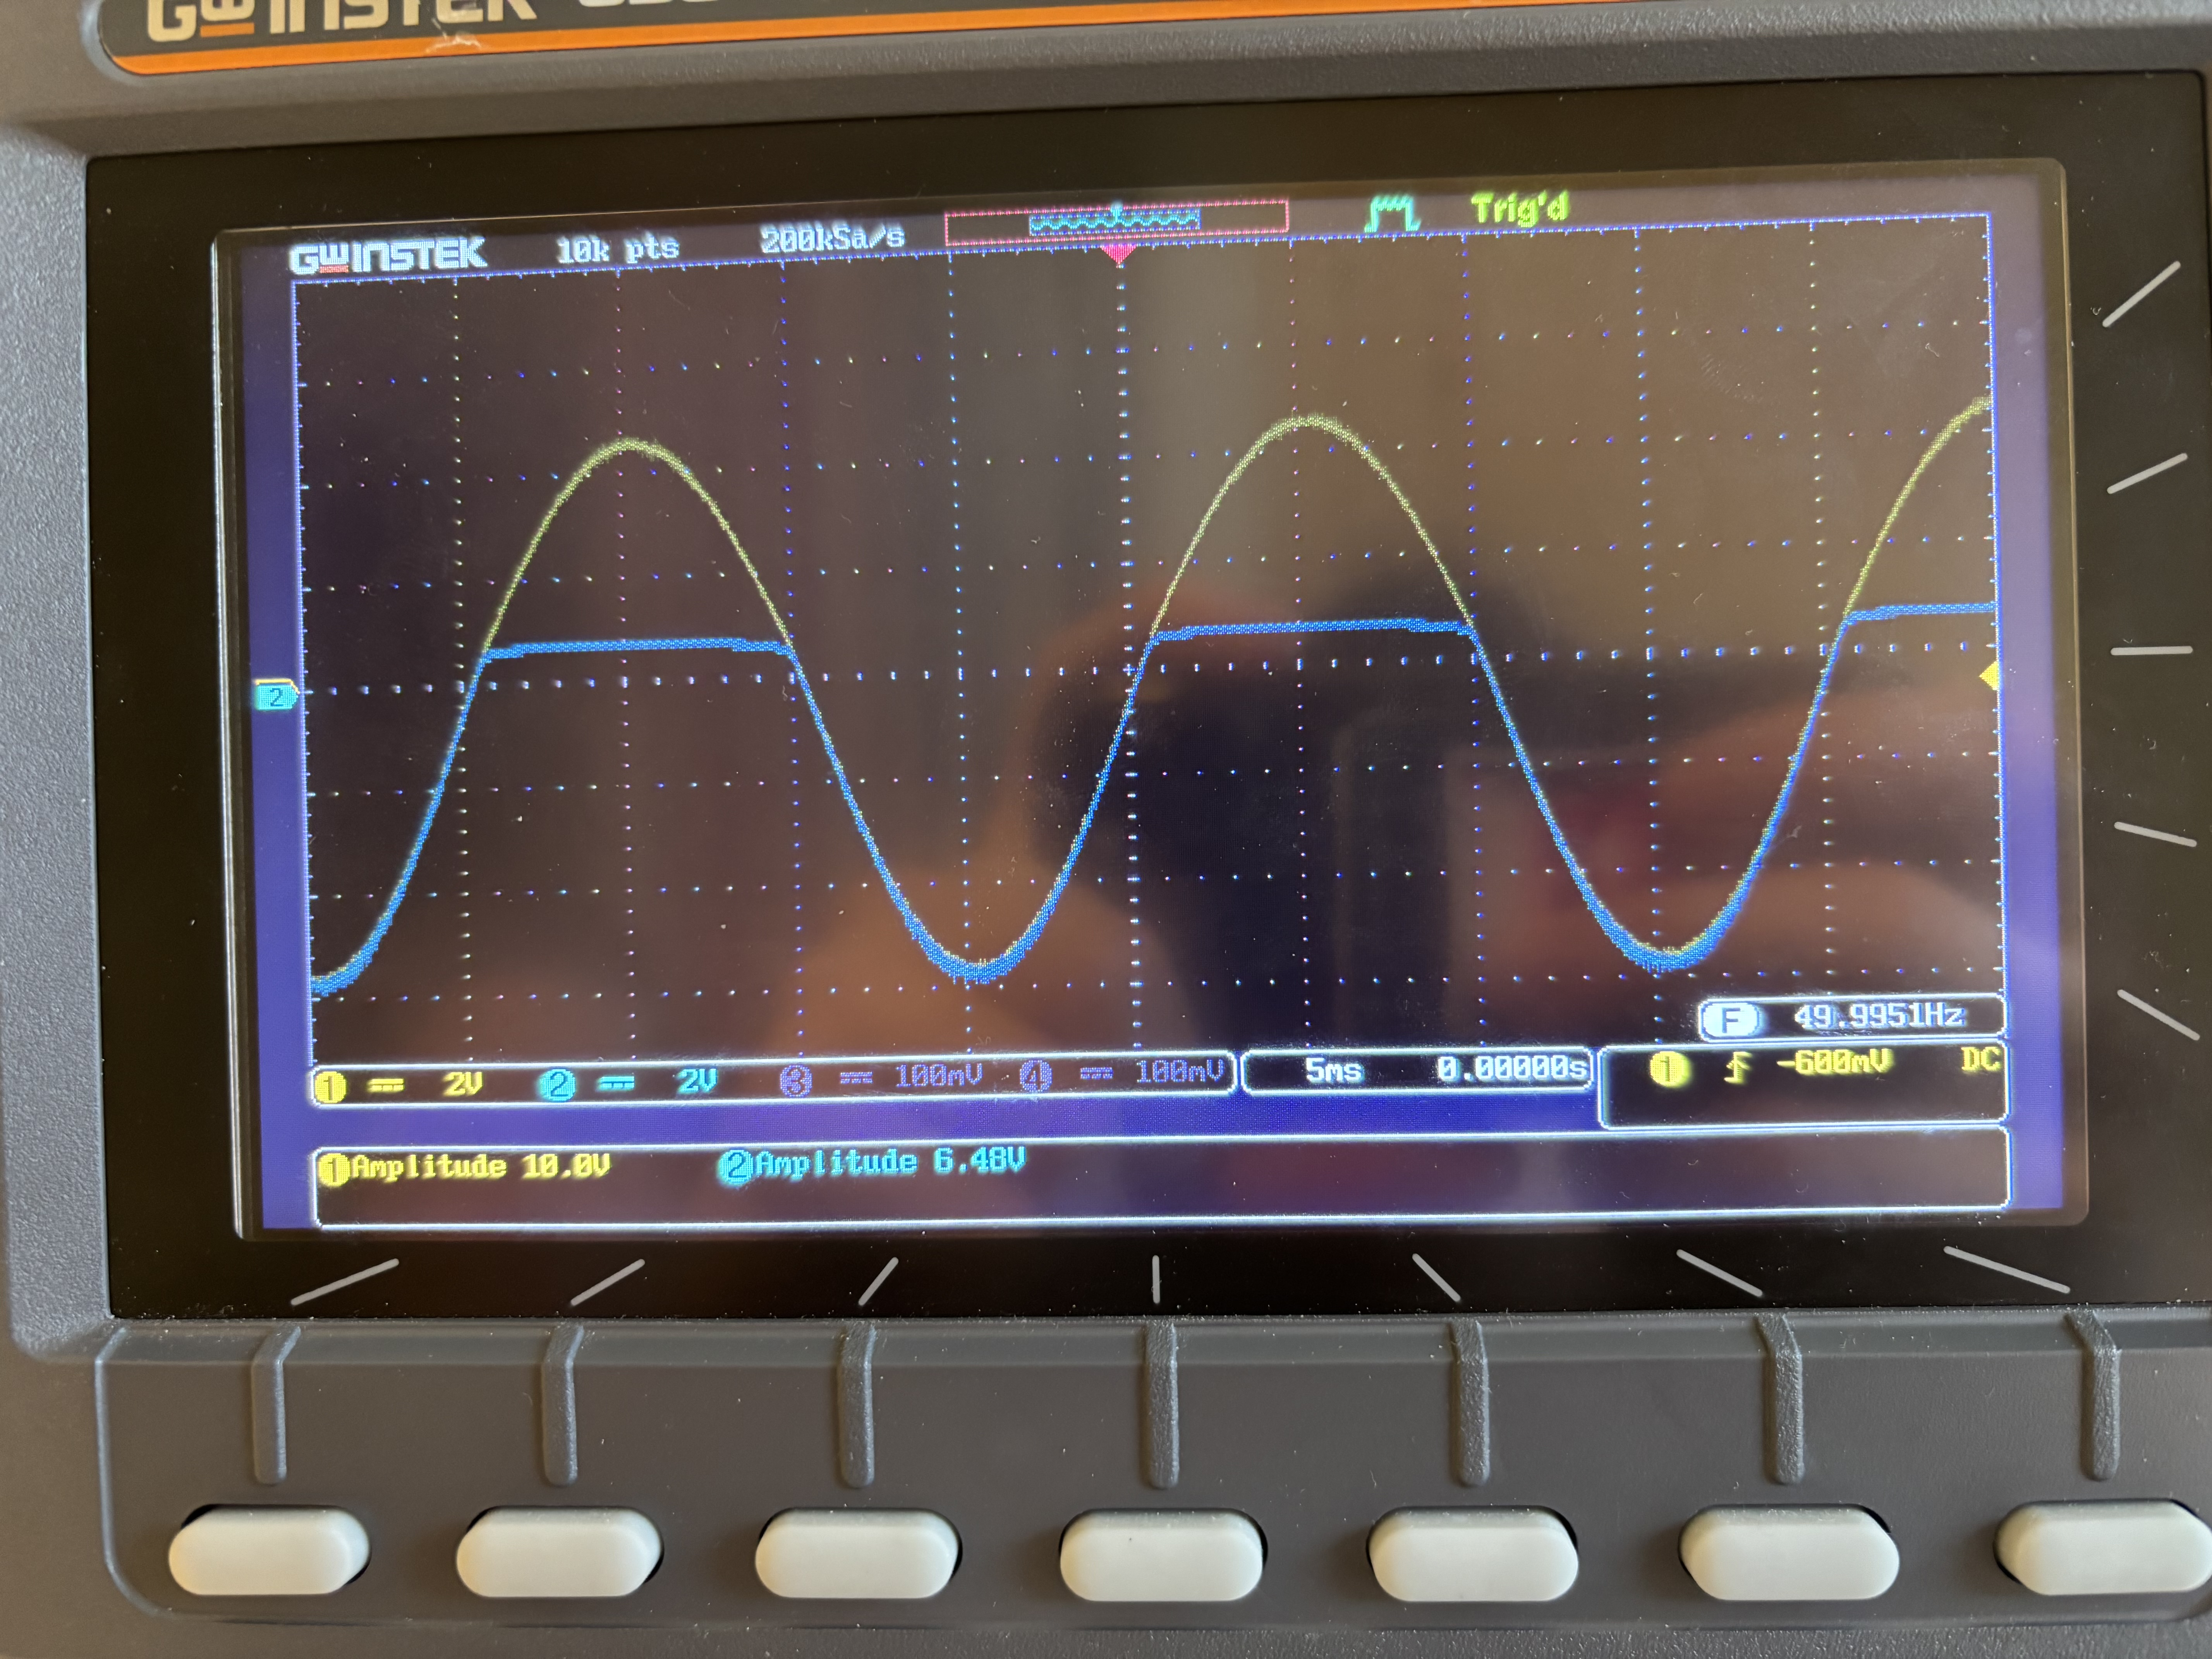
\includegraphics[width=0.85\textwidth]{Media/krets1.jpg}
    \caption{Oscilloskopbilde av utgangsspenning i krets 1}\label{fig:krets1-oscillskop}
\end{figure}


\begin{figure}[H]
\centering
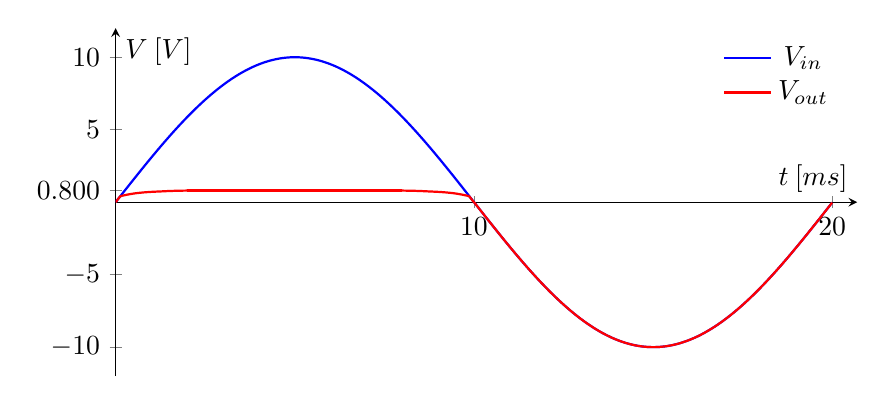
\begin{tikzpicture}
\begin{axis}[
    width=11cm,
    height=6cm,
    axis lines=middle,
    xlabel={$t\:[ms]$},
    ylabel={$V\:[V]$},
    xmin=0, xmax=6.5,
    ymin=-12, ymax=12,
    samples=400,
    domain=0:6.28,
    ytick={-10,-5,0.8,5,10},
    yticklabels={$-10$, $-5$, $0.800$, $5$, $10$},
    xtick={3.14,6.28},
    xticklabels={$10$, $20$},
    legend style={
        at={(0.98,0.98)},
        anchor=north east,
        draw=none,
        fill=none
    }
]

% Inngangsspenning
\addplot[
    blue,
    thick
] {10*sin(deg(x))};
\addlegendentry{$V_{in}$}

\addplot[
    red,
    thick,
    domain=3.14:6.28
] {10*sin(deg(x))};

% Utgangsspenning med styrt, glatt klipping
\addplot[
    red,
    thick,
    smooth,
] coordinates {
    (0.00, 0.00)
    (0.01, 0.10)
    (0.02, 0.20)
    (0.03, 0.30)
    (0.04, 0.40)
    (0.06, 0.45)
    (0.09, 0.50)
    (0.13, 0.56)
    (0.18, 0.62)
    (0.24, 0.67)
    (0.31, 0.71)
    (0.39, 0.74)
    (0.47, 0.77)
    (0.55, 0.79)
    (0.63, 0.80)
};
\addlegendentry{$V_{out}$}

\addplot[
    red,
    thick
] coordinates {(0.63, 0.80) (2.51, 0.80)};

\addplot[
    red,
    thick,
    smooth,
] coordinates {
    (2.51, 0.80)
    (2.55, 0.795)
    (2.59, 0.79)
    (2.67, 0.77)
    (2.75, 0.74)
    (2.83, 0.71)
    (2.90, 0.67)
    (2.96, 0.62)
    (3.01, 0.56)
    (3.05, 0.50)
    (3.08, 0.45)
    (3.10, 0.40)
    (3.11, 0.30)
    (3.12, 0.20)
    (3.13, 0.10)
    (3.14, 0.00)
};

\end{axis}
\end{tikzpicture}
\caption{Måleresultat for krets 1.}\label{fig:resultat_krets1}
\end{figure}

\paragraph{Kommentar til resultatet. } Utgangsspenningen klippes ved $800\mathrm{mV}$ (målt med cursors på oscilloskopet), som er omtrent det vi forventer for en silisiumdiode. Den negative halvbølgen følger inngangsspenningen. Måleresultatet for denne kretsen er som forventet og har ingen store avvik fra det teoretiske resultatet.

\subsection{Krets 2 -- toveis klippekrets}
For å koble opp kretsen benytter vi komponentene i krets 2 (se figur~\ref{fig:krets2}). Signalgeneratoren bruker innstillingen for en sinusformet spenning med toppverdi $10\mathrm{V}$ og frekvens $50\mathrm{Hz}$. Vi bruker en motstand på $180\Omega$ i serie med to parallellkoblet dioder. Diodene skal være orientert i motstatt retning av hverandre. Oscilloskopet bruker en kanal for å måle inngangsspenningen, og en kanal for å måle over diodene.

\vspace{2em}

\begin{figure}[H]
    \centering
    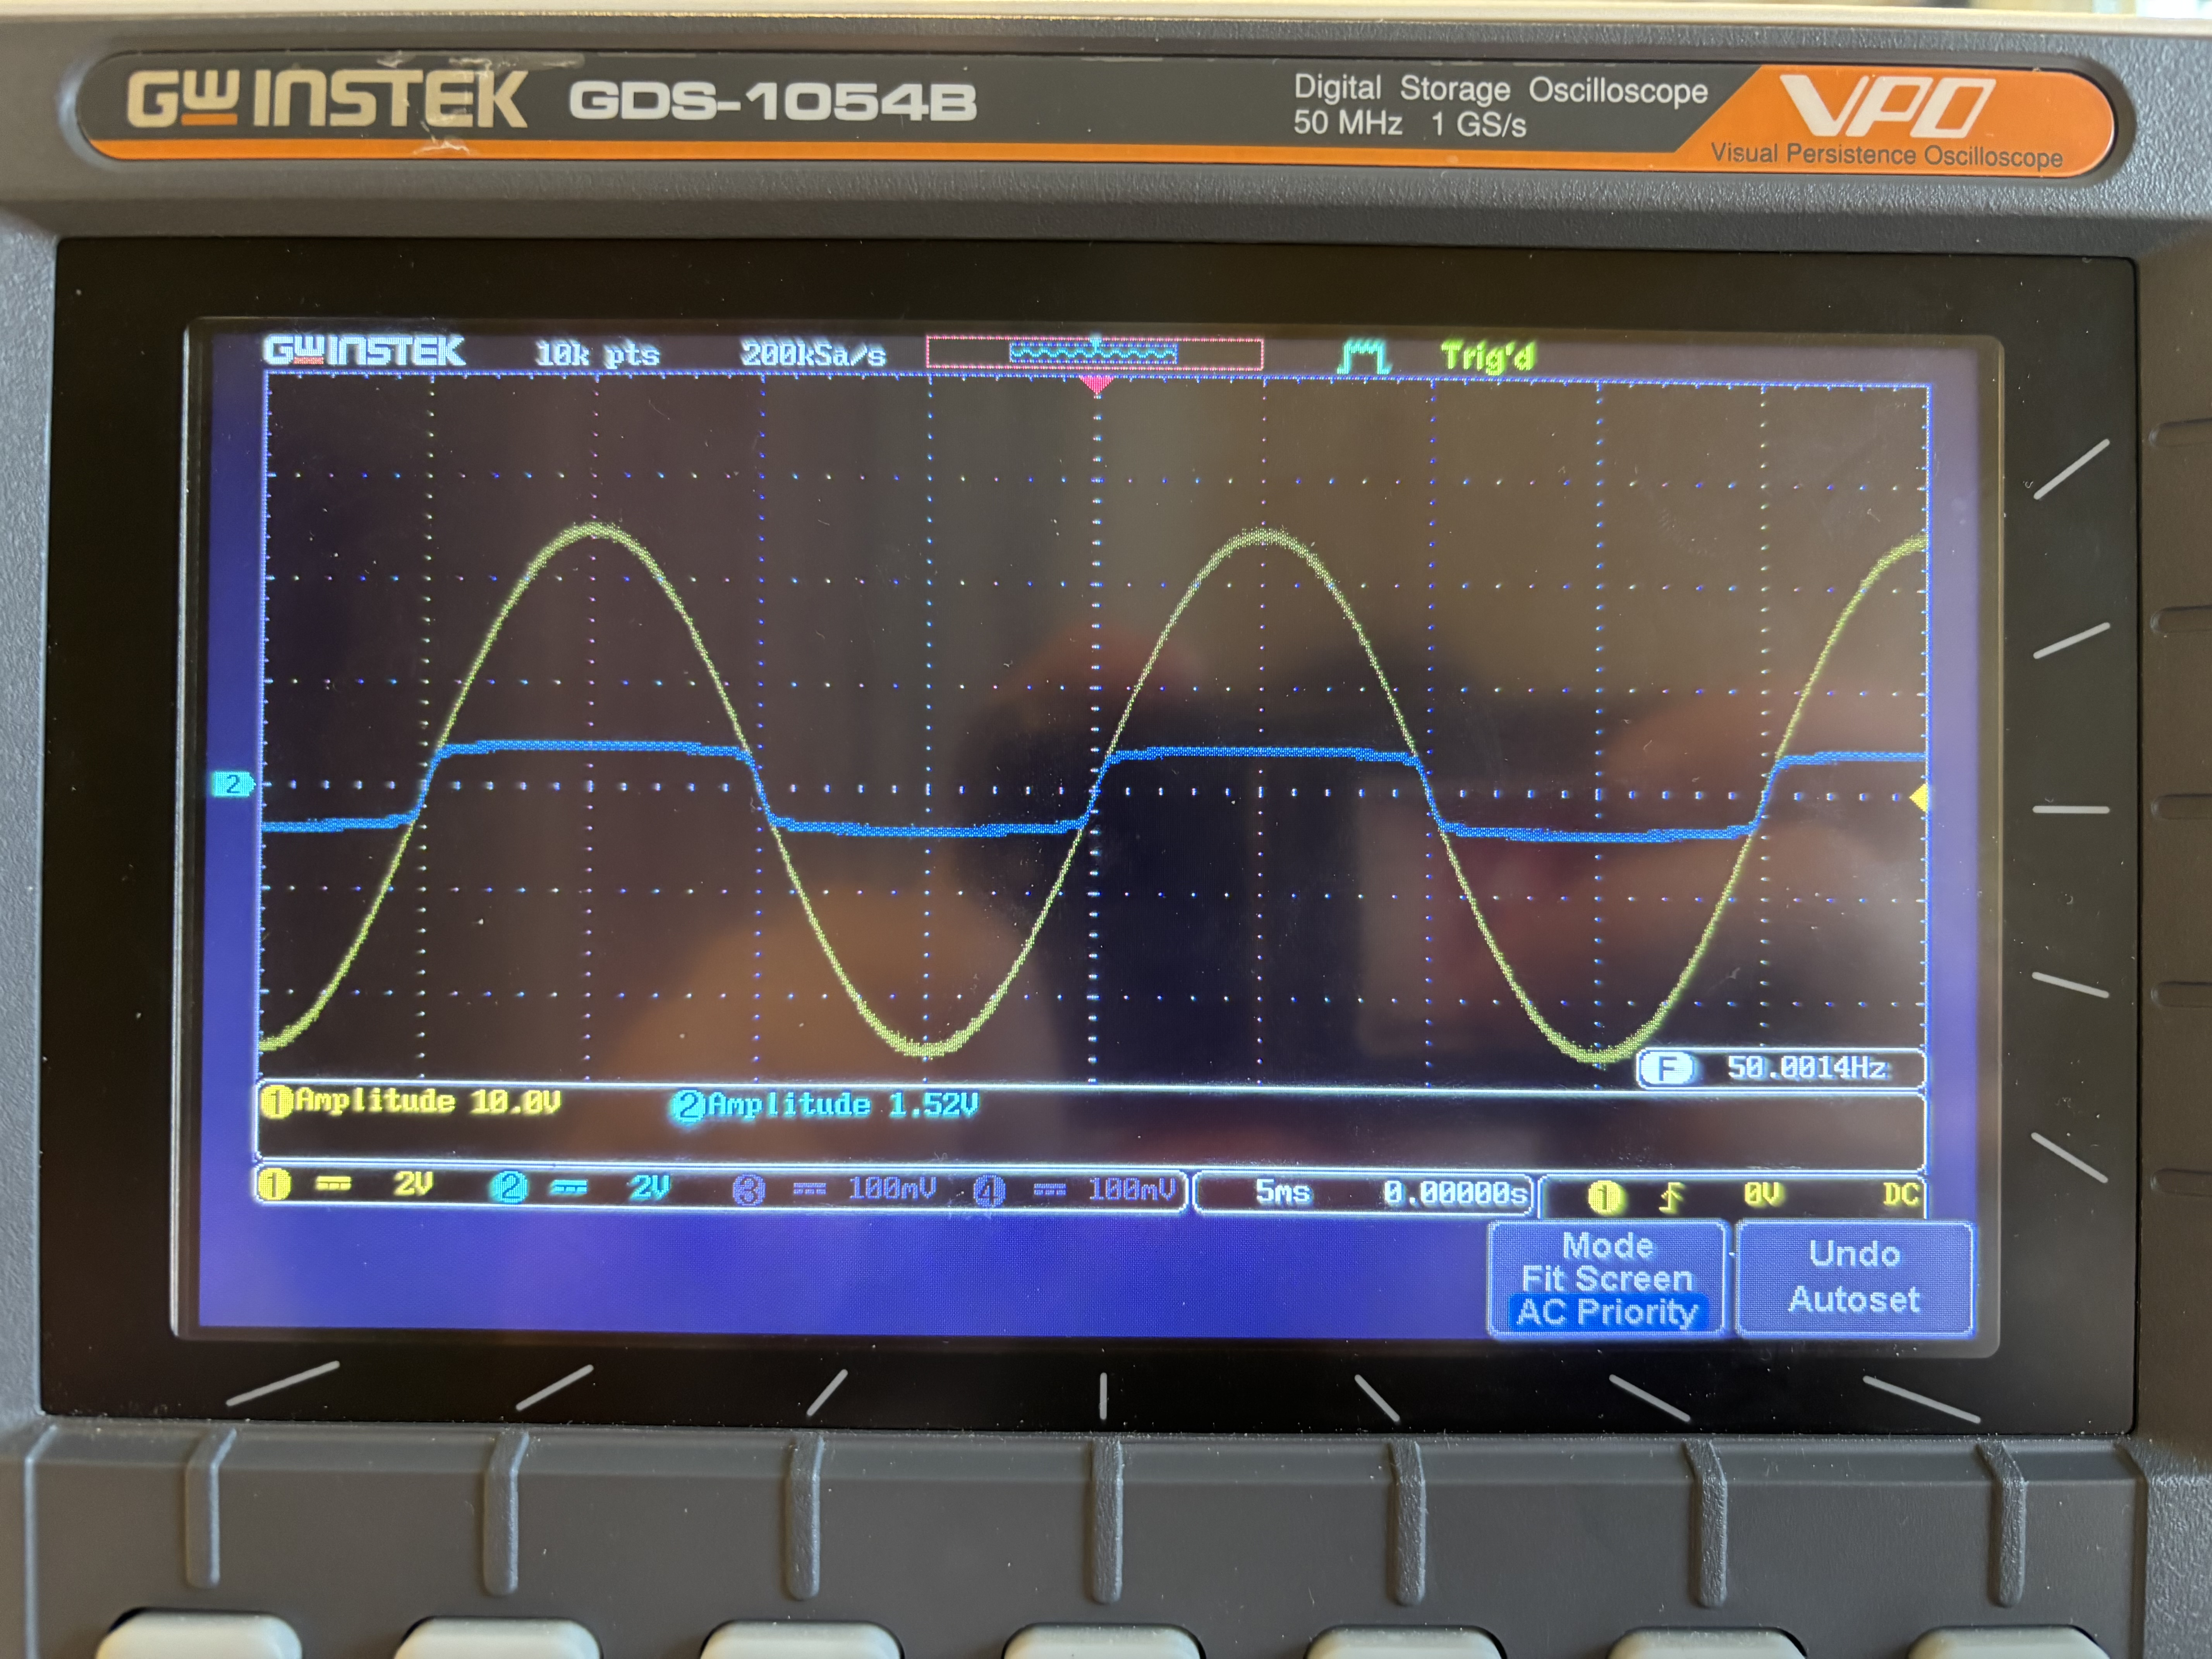
\includegraphics[width=0.85\textwidth]{Media/krets2.jpg}
    \caption{Oscilloskopbilde av utgangsspenning i krets 2}\label{fig:krets2-oscillskop}
\end{figure}


\begin{figure}[H]
\centering
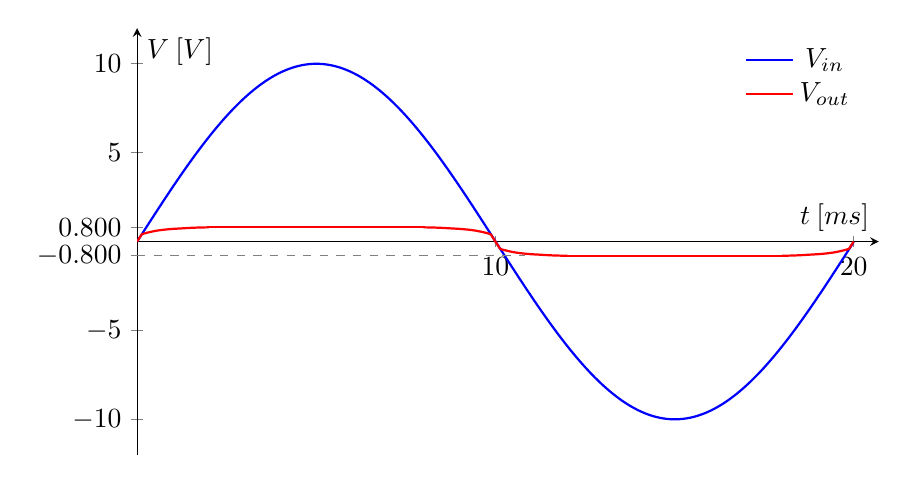
\begin{tikzpicture}
\begin{axis}[
    width=11cm,
    height=7cm,
    axis lines=middle,
    xlabel={$t\:[ms]$},
    ylabel={$V\:[V]$},
    xmin=0, xmax=6.5,
    ymin=-12, ymax=12,
    samples=400,
    domain=0:6.28,
    ytick={-10,-5,-0.8,0.8,5,10},
    yticklabels={$-10$, $-5$, $-0.800$, $0.800$, $5$, $10$},
    xtick={3.14,6.28},
    xticklabels={$10$, $20$},
    legend style={
        at={(0.98,0.98)},
        anchor=north east,
        draw=none,
        fill=none
    }
]

% Inngangsspenning
\addplot[
    blue,
    thick
] {10*sin(deg(x))};
\addlegendentry{$V_{in}$}

% -------- POSITIV HALVPERIODE --------

\addplot[
    red,
    thick,
    smooth
] coordinates {
    (0.00, 0.00)
    (0.01, 0.10)
    (0.02, 0.20)
    (0.03, 0.30)
    (0.04, 0.40)
    (0.06, 0.45)
    (0.09, 0.50)
    (0.13, 0.56)
    (0.18, 0.62)
    (0.24, 0.67)
    (0.31, 0.71)
    (0.39, 0.74)
    (0.47, 0.77)
    (0.55, 0.79)
    (0.63, 0.80)
};

\addplot[
    red,
    thick
] coordinates {(0.63, 0.80) (2.51, 0.80)};

\addplot[
    red,
    thick,
    smooth
] coordinates {
    (2.51, 0.80)
    (2.55, 0.795)
    (2.59, 0.79)
    (2.67, 0.77)
    (2.75, 0.74)
    (2.83, 0.71)
    (2.90, 0.67)
    (2.96, 0.62)
    (3.01, 0.56)
    (3.05, 0.50)
    (3.08, 0.45)
    (3.10, 0.40)
    (3.11, 0.30)
    (3.12, 0.20)
    (3.13, 0.10)
    (3.14, 0.00)
};

% -------- NEGATIV HALVPERIODE (speilet) --------

\addplot[
    red,
    thick,
    smooth
] coordinates {
    (3.14, 0.00)
    (3.15, -0.10)
    (3.16, -0.20)
    (3.17, -0.30)
    (3.18, -0.40)
    (3.20, -0.45)
    (3.23, -0.50)
    (3.27, -0.56)
    (3.32, -0.62)
    (3.38, -0.67)
    (3.45, -0.71)
    (3.53, -0.74)
    (3.61, -0.77)
    (3.69, -0.79)
    (3.77, -0.80)
};

\addplot[
    red,
    thick
] coordinates {(3.77, -0.80) (5.65, -0.80)};

\addplot[
    red,
    thick,
    smooth
] coordinates {
    (5.65, -0.80)
    (5.69, -0.795)
    (5.73, -0.79)
    (5.81, -0.77)
    (5.89, -0.74)
    (5.97, -0.71)
    (6.04, -0.67)
    (6.10, -0.62)
    (6.15, -0.56)
    (6.19, -0.50)
    (6.22, -0.45)
    (6.24, -0.40)
    (6.25, -0.30)
    (6.26, -0.20)
    (6.27, -0.10)
    (6.28, 0.00)
};

% Klippelinjer
%\addplot[dashed, gray] coordinates {(0,0.8) (6.28,0.8)};
\addplot[dashed, gray] coordinates {(0,-0.8) (3.40,-0.8)};

\addlegendentry{$V_{out}$}

\end{axis}
\end{tikzpicture}
\caption{Måleresultat for krets 2.}\label{fig:resultat_krets2}
\end{figure}

\paragraph{Kommentar til resultatet. } Utgangsspenningen klippes ved $800\mathrm{mV}$ både i den positive og negative halvbølgen (målt med cursors på oscilloskopet), som er det vi omtrent forventer for en silisiumdiode. Resultatet her har samme praktiske måling som i krets 1, som betyr at det samsvarer på tvers av kretser. Måleresultatet for denne kretsen er som forventet og har ingen store avvik fra teoretiske forventninger.

\subsection{Krets 3 -- zenordioder i klippekrets}

Signalgeneratoren bruker innstillingene for en sinusformet spenning med toppverdi $10\mathrm{V}$ og frekvens $50\mathrm{Hz}$. Vi bruker en motstand på $180\Omega$ i serie med to zenordioder. Den ene zenordioden har zenorspenning på $4.7\mathrm{V}$ og den andre har zenorspenning på $6.8\mathrm{V}$. Diodene skal være plassert og orientert slik i kretsfremstillingen i figur~\ref{fig:krets3}. Oscilloskopet bruker en kanal for å måle inngangsspenningen, og en kanal for å måle over zenordiodene i serie.

\begin{figure}[H]
    \centering
    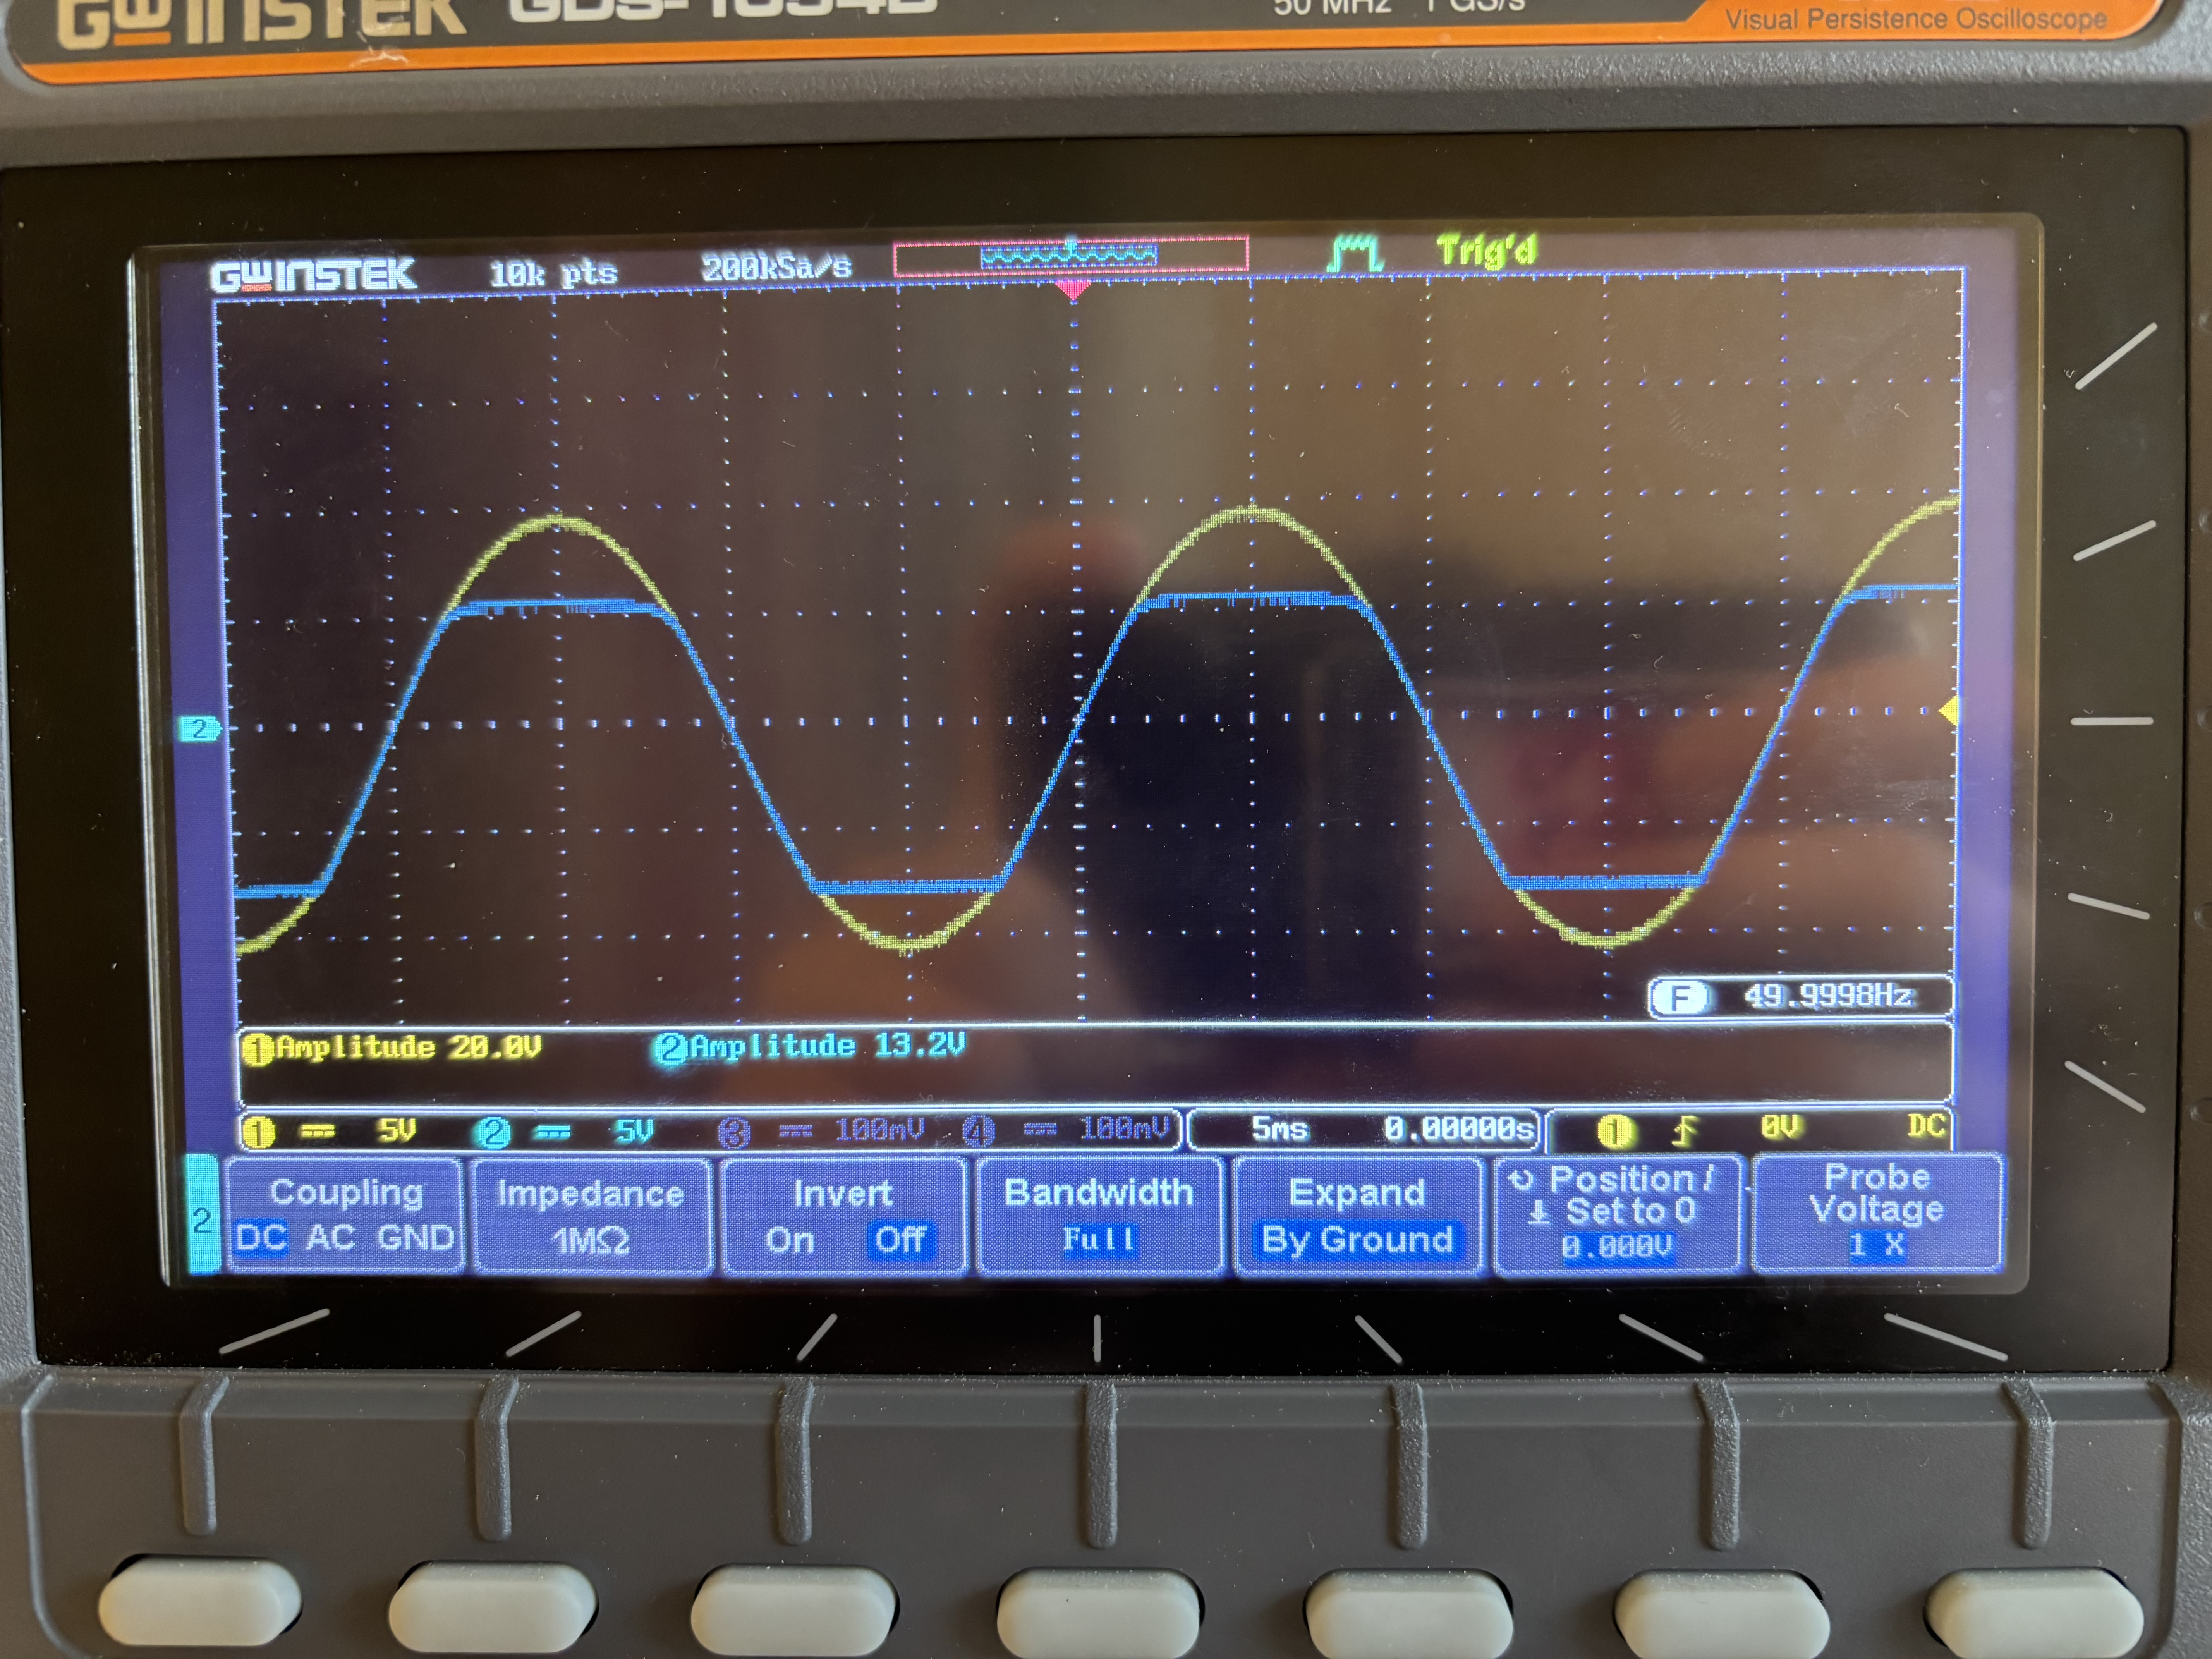
\includegraphics[width=0.80\textwidth]{Media/krets3.jpg}
    \caption{Oscilloskopbilde av utgangsspenning i krets 3}\label{fig:krets3-oscillskop}
\end{figure}


\begin{figure}[H]
\centering
\begin{tikzpicture}
\begin{axis}[
    width=11cm,
    axis lines=middle,
    xlabel={$t\:[ms]$},
    ylabel={$V\:[V]$},
    xmin=0, xmax=6.5,
    ymin=-12, ymax=12,
    samples=300,
    domain=0:6.28,
    ytick={-10,-7.60,-5,0,5.60,10},
    yticklabels={$-10$, $-7.60$, $-5$, $0$, $5.60$, $10$},
    xtick={3.14,6.28},
    xticklabels={$10$, $20$},
    legend style={
        at={(0.98,0.98)},
        anchor=north east,
        draw=none,
        fill=none
    }
]

% Inngangsspenning
\addplot[
    blue,
    thick
] {10*sin(deg(x))};
\addlegendentry{$V_{in}$}

% Utgangsspenning: stigende positiv del
\addplot[
    red,
    thick,
    smooth
] coordinates {
    (0.00, 0.00)
    (0.10, 1.00)
    (0.20, 2.00)
    (0.35, 3.40)
    (0.50, 4.60)
    (0.63, 5.20)
    (0.75, 5.45)
    (0.90, 5.58)
    (1.00, 5.60)
};
\addlegendentry{$V_{out}$}

% Utgangsspenning: platå positiv
\addplot[
    red,
    thick
] coordinates {
    (1.00, 5.60)
    (2.14, 5.60)
};

% Utgangsspenning: fallende positiv del
\addplot[
    red,
    thick,
    smooth
] coordinates {
    (2.14, 5.60)
    (2.24, 5.58)
    (2.39, 5.45)
    (2.51, 5.20)
    (2.64, 4.60)
    (2.79, 3.40)
    (2.94, 2.00)
    (3.04, 1.00)
    (3.14, 0.00)
};

% Utgangsspenning: negativ sinus fram til klipping
\addplot[
    red,
    thick,
    domain=3.14:4.00
] {10*sin(deg(x))};

% Utgangsspenning: flatt negativt platå
\addplot[
    red,
    thick
] coordinates {
    (4.00, -7.60)
    (5.42, -7.60)
};

% Utgangsspenning: følger sinus opp igjen
\addplot[
    red,
    thick,
    domain=5.42:6.28
] {10*sin(deg(x))};

% Hjelpelinjer
\addplot[
    dashed,
    gray
] coordinates {(0,5.60) (0.85,5.60)};

\addplot[
    dashed,
    gray
] coordinates {(0,-7.60) (4,-7.60)};

\end{axis}
\end{tikzpicture}
\caption{Måleresultat for krets 3.}
\label{fig:resultat_krets3}
\end{figure}

\paragraph{Kommentar til resultat. } Utgangsspenningen klippes ved $5.60\mathrm{V}$ i den positive halvbølgen og ved $-7.60\mathrm{V}$ i den negative halvbølgen (begge målinger er målt med cursors på oscilloskopet). Måleresultatet er som forventet og har ingen store avvik fra det teoretiske resultatet.

\subsection{Krets 4 -- enveis likeretter}

I denne delen av forsøket kobler vi opp krets 4 (se figur~\ref{fig:krets4}). Signalgeneratoren bruker innstillingene for en sinusformet spenning med toppverdi $10\mathrm{V}$ og frekvens $50\mathrm{Hz}$. Vi bruker en motstand på $1\mathrm{k\Omega}$ i serie med en diode. Dioden og motstanden plasseres slik i kretsen. Oscilloskopet bruker en kanal for å måle inngangsspenningen fra signalgeneratoren, og en kanal over motstanden. Måleresultatet for den positive likeretteren kommer når dioden er orientert som i krets 4, og måleresultatet for den negative likeretteren kommer når dioden er snudd i forhold til krets 4. Resultatene er i figurene under.

\begin{figure}[H]
\centering

\begin{subfigure}{0.48\textwidth}
    \centering
    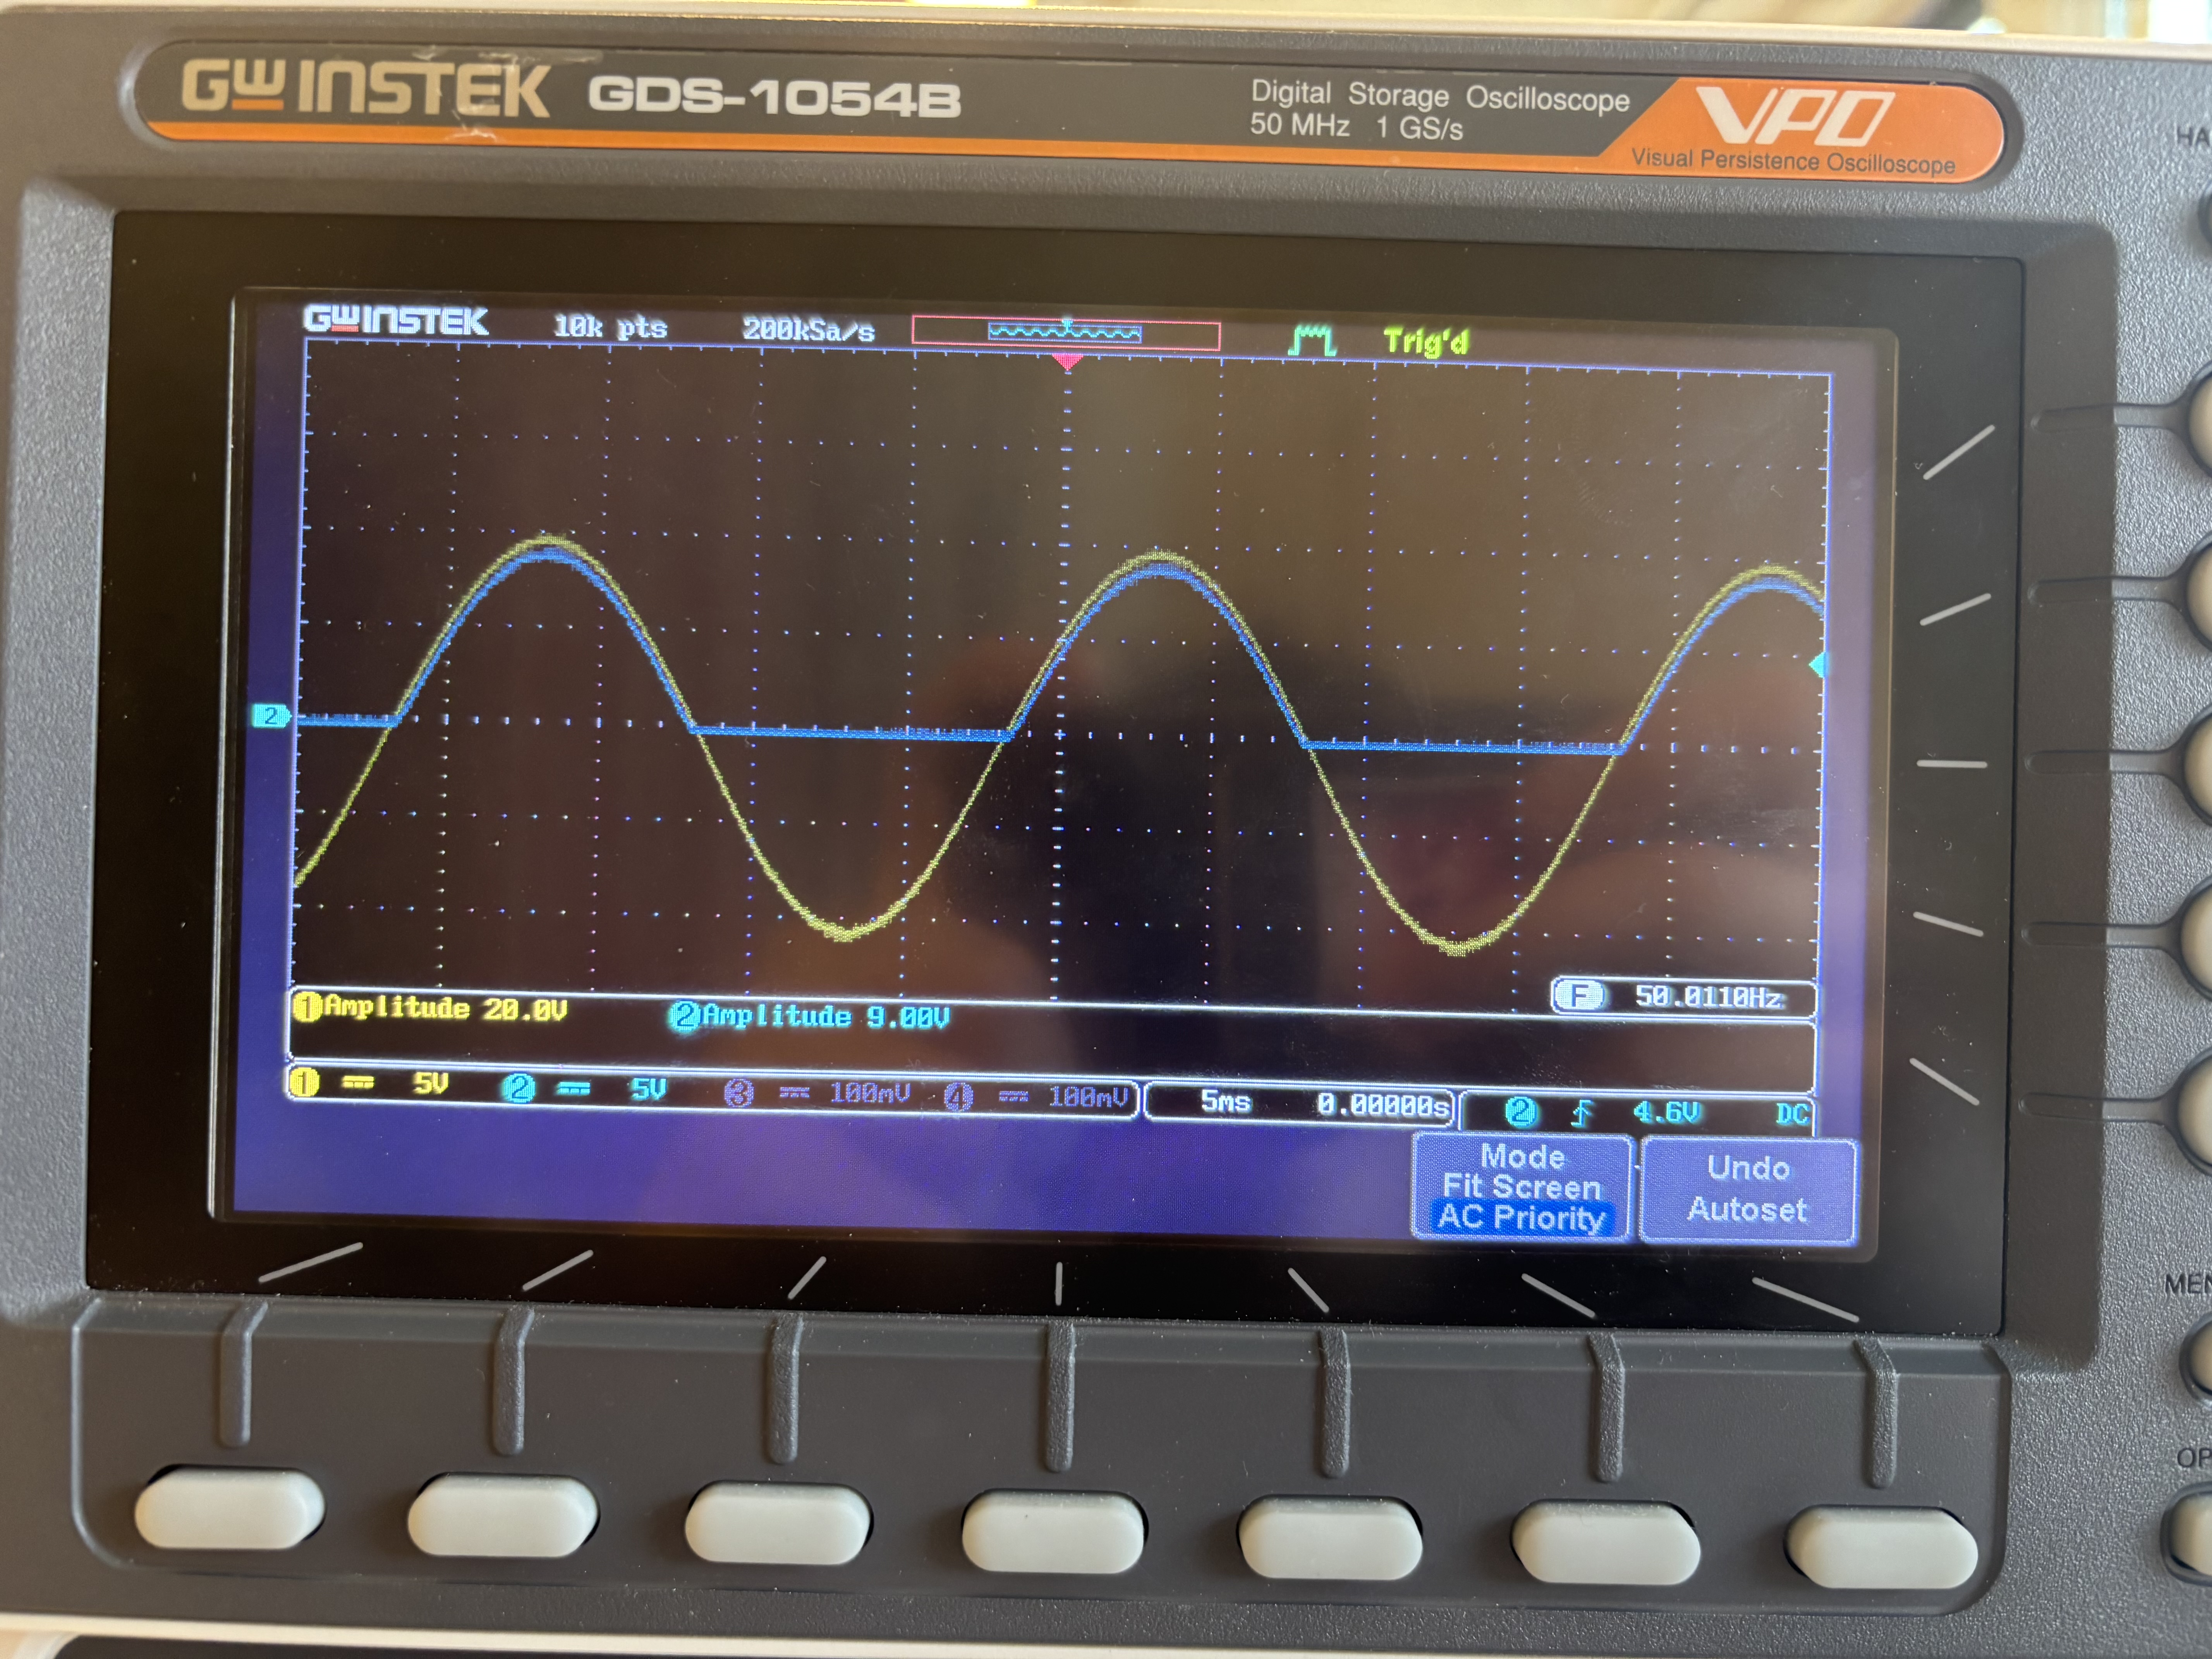
\includegraphics[width=\linewidth]{Media/krets4_pos.jpg}
    \caption{Positiv halvbølge}
    \label{fig:krets4_pos-oscillskop}
\end{subfigure}
\hfill
\begin{subfigure}{0.48\textwidth}
    \centering
    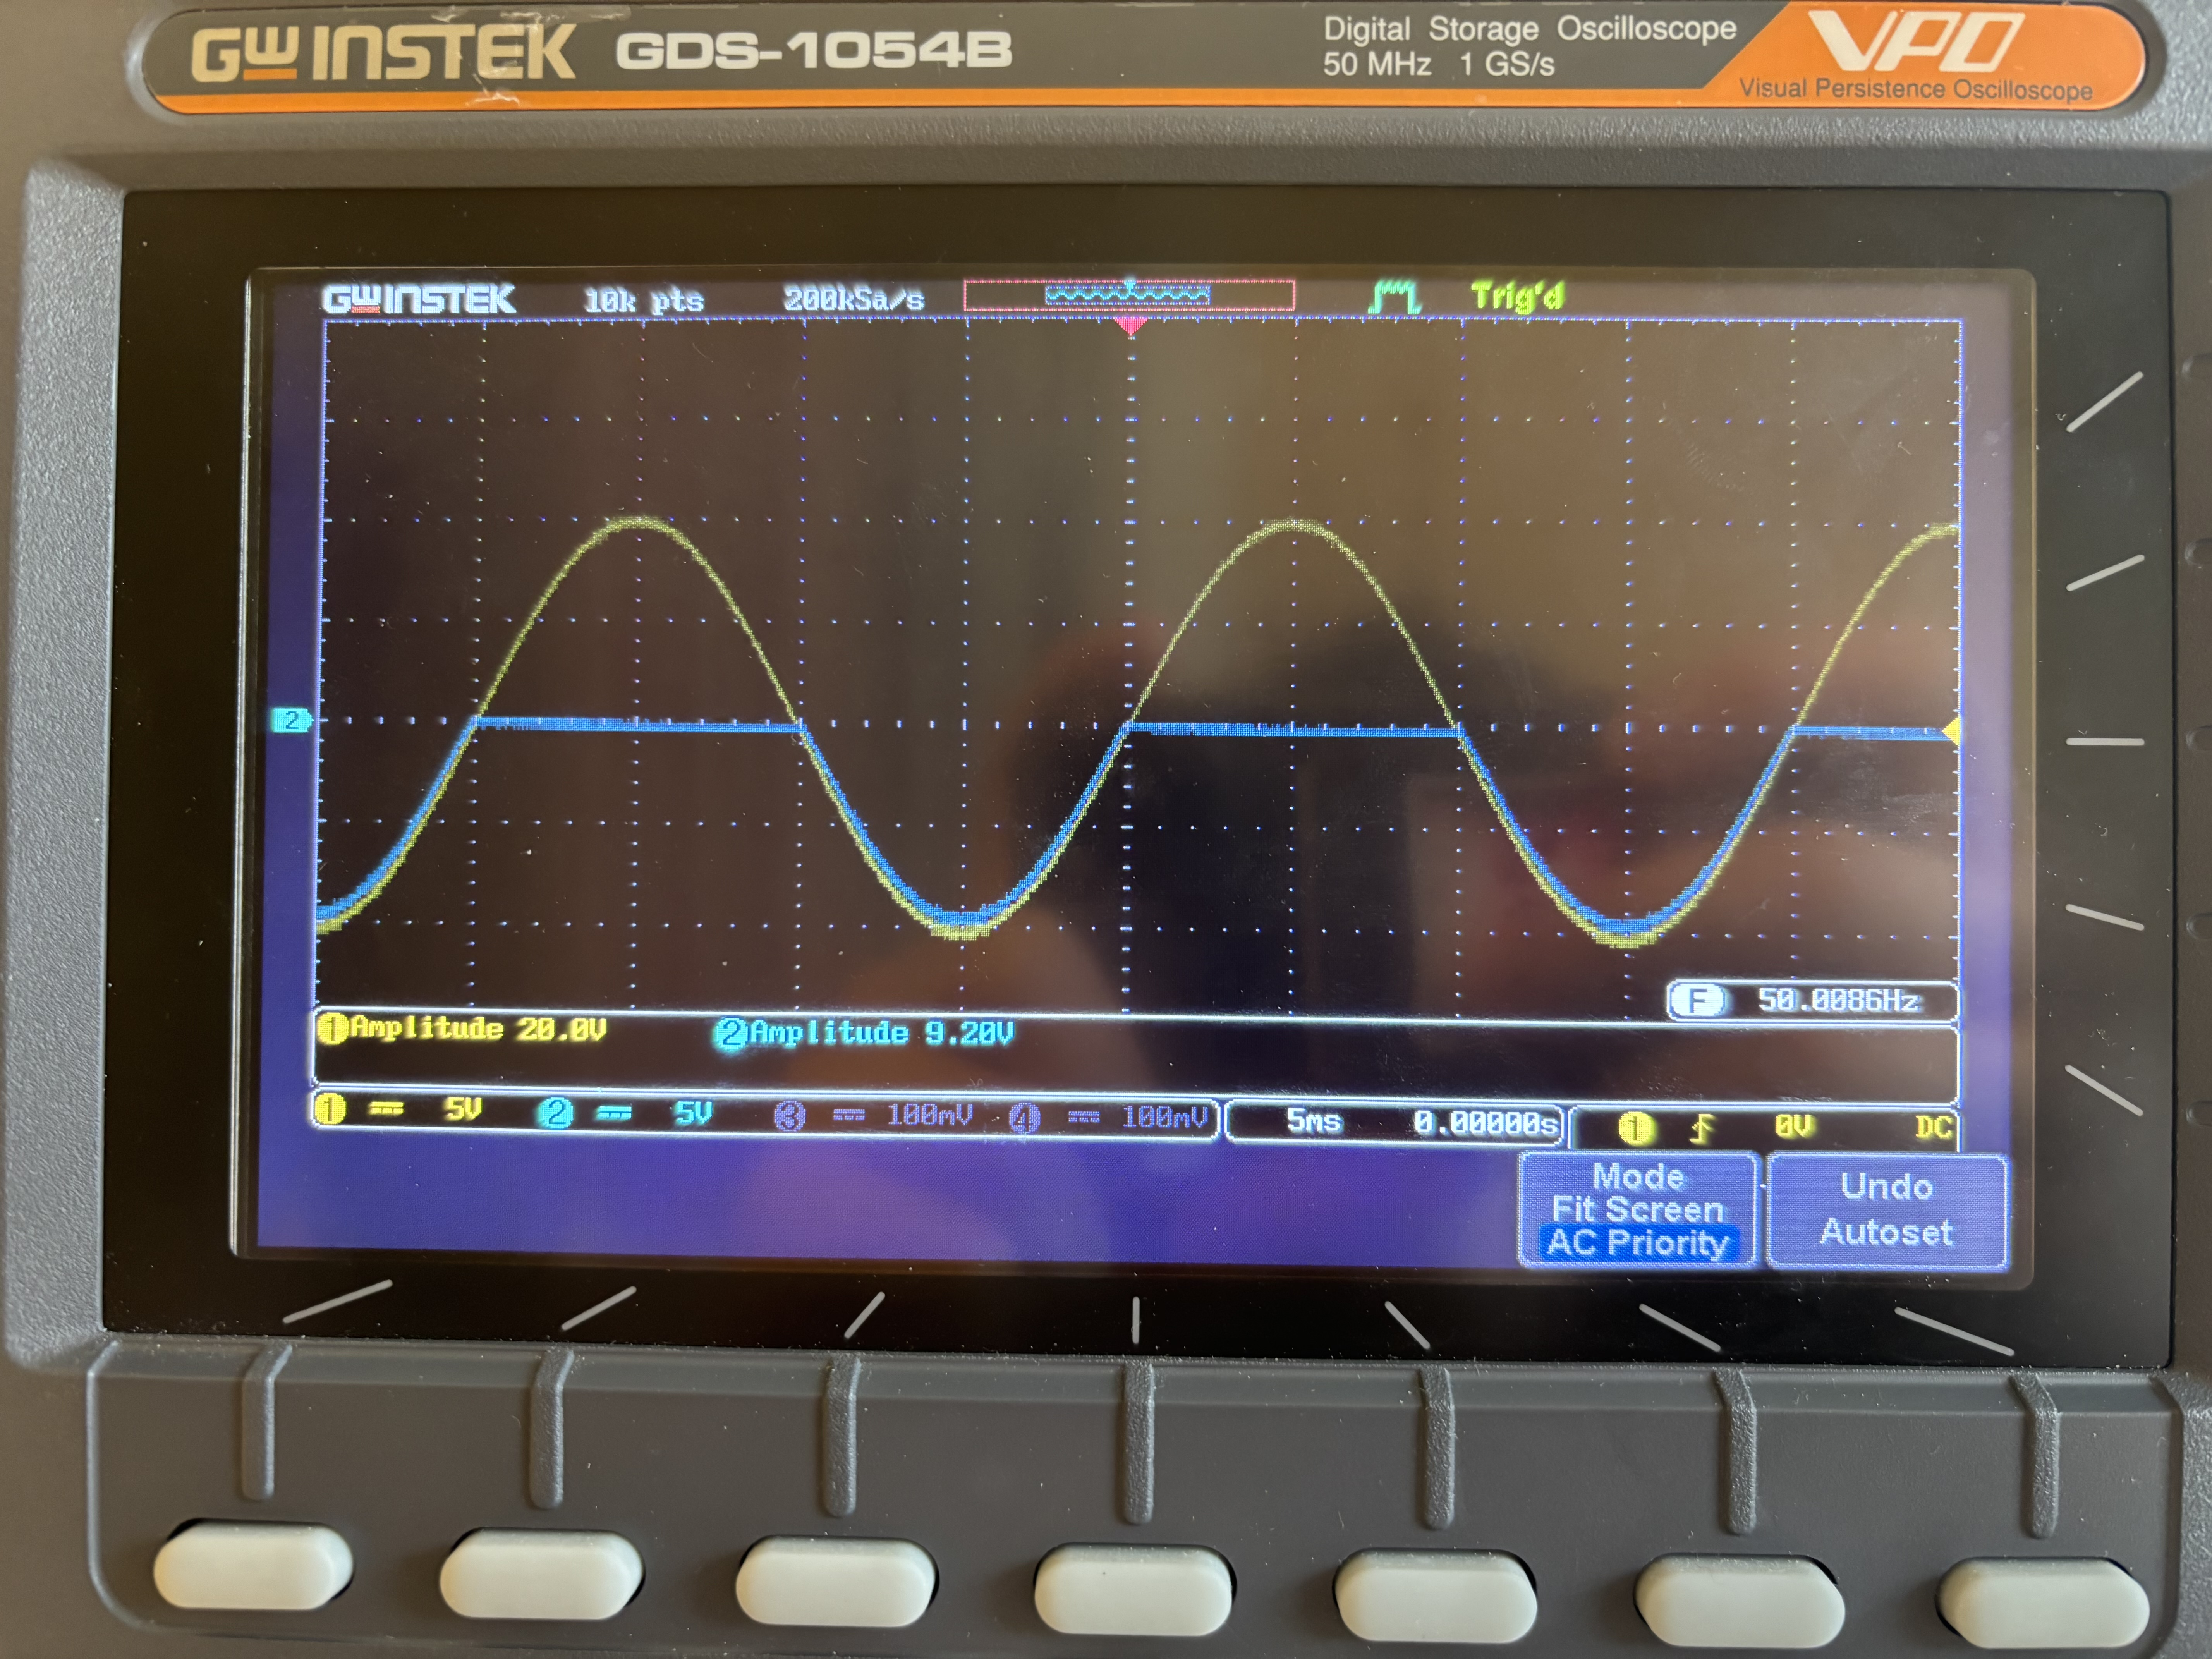
\includegraphics[width=\linewidth]{Media/krets4_neg.jpg}
    \caption{Negativ halvbølge}
    \label{fig:krets4_neg-oscillskop}
\end{subfigure}

\caption{Oscilloskopbilder av utgangsspenning i krets 4}
\label{fig:krets4_oscilloskop}
\end{figure}


\begin{figure}[H]
\centering

\begin{subfigure}{0.48\textwidth}
\centering
\begin{tikzpicture}
\begin{axis}[
    width=\linewidth,
    axis lines=middle,
    xlabel={$t\:[ms]$},
    ylabel={$V\:[V]$},
    xmin=0, xmax=6.5,
    ymin=-12, ymax=12,
    samples=300,
    domain=0:6.28,
    ytick={-10,-5,0,5,9},
    yticklabels={$-10$, $-5$, $0$, $5$, $9.0$},
    xtick={3.14,6.28},
    xticklabels={$10$, $20$},
    legend style={
        at={(0.98,0.98)},
        anchor=north east,
        draw=none,
        fill=none
    }
]

\addplot[blue, thick] {10*sin(deg(x))};
\addplot[red, thick] {max(10*sin(deg(x)) -0.6 - 0.4*sin(deg(x)), 0)};

\addplot[dashed, gray] coordinates {(0,9) (1.57,9)};

\end{axis}
\end{tikzpicture}
\caption{Positiv enveis likeretter}\label{fig:resultat_krets4_diode_positiv}
\end{subfigure}
\hfill
\begin{subfigure}{0.48\textwidth}
\centering
\begin{tikzpicture}
\begin{axis}[
    width=\linewidth,
    axis lines=middle,
    xlabel={$t\:[ms]$},
    ylabel={$V\:[V]$},
    xmin=0, xmax=6.5,
    ymin=-12, ymax=12,
    samples=300,
    domain=0:6.28,
    ytick={-9.20,-5,0,5,10},
    yticklabels={$-9.20$, $-5$, $0$, $5$, $10$},
    xtick={3.14,6.28},
    xticklabels={$10$, $20$},
    legend style={
        at={(0.98,0.98)},
        anchor=north east,
        draw=none,
        fill=none
    }
]

\addplot[blue, thick] {10*sin(deg(x))};
\addplot[red, thick] {min(10*sin(deg(x)) +0.6 - 0.20*sin(deg(x)), 0)};

\addplot[dashed, gray] coordinates {(0,-9.20) (4.71,-9.20)};

\end{axis}
\end{tikzpicture}
\caption{Negativ enveis likeretter}\label{fig:resultat_krets4_diode_negativ}
\end{subfigure}

\caption{Måleresultater krets 4.}
\label{fig:resultat_krets4_diode_begge}

\end{figure}

\noindent
I tillegg måler vi DC-verdien i begge tilfeller. Dette utføres med å bruke et multimeter i DC-spenningsmålemodus, som kobles over motstanden i kretsen. Resultatene for både positiv og negativ likeretter er i tabellen under.

\begin{table}[H]
\centering
\caption{Resultater for DC-verdier i krets 4.}
\label{tab:krets4_dc_verdier}
\begin{tabular}{lccc}
\toprule
\textbf{Komponent} & \textbf{Teoretisk verdi} & \textbf{Målt verdi} & \textbf{Avvik [\%]} \\
\midrule

% --- Fyll inn rader her ---
% Eksempel:
$V_{DC} \: \left(+\right)$ & $2.84\text{V}$ & $2.73\text{V}$ & 3.87\% \\
$V_{DC} \: \left(-\right)$ & $-2.84\text{V}$ & $-2.83\text{V}$ & 0.35\% \\


% Du kan også lage grupper med tom linje hvis ønskelig

\bottomrule
\end{tabular}
\end{table}

\paragraph{Kommentar til resultater. } Likeretteren for positiv halvbølge har noe større avvik enn likeretteren for negativ halvbølge. Dette gjenspeiler seg også i DC-verdiene, hvor den positive likeretteren har et avvik på 3.87\%, mens den negative likeretteren har et avvik på 0.35\%. Måleresultatene for begge likeretterne er likevel i rimelig god overensstemmelse med det teoretiske resultatet, og det er ingen store avvik som indikerer feil i oppkoblingen eller målefeil.


\subsection{Krets 5 -- toveis likeretter}

For å oppnå formålet med en toveis likeretter, benytter vi teorien for en enkel diodebro og kobler opp krets 5 (se figur~\ref{fig:krets5}). Signalgeneratoren bruker innstillingene for en sinusformet spenning med toppverdi $10\mathrm{V}$ og frekvens $50\mathrm{Hz}$. Vi bruker en motstand på $1\mathrm{k\Omega}$ i serie med fire dioder som er koblet i en brokonfigurasjon slik som i teori for toveis likeretter (se seksjon~\ref{teo:toveis_likeretter}). Oscilloskopet bruker en kanal for å måle inngangsspenningen, og en kanal for å måle over motstanden.

\begin{figure}[H]
    \centering
    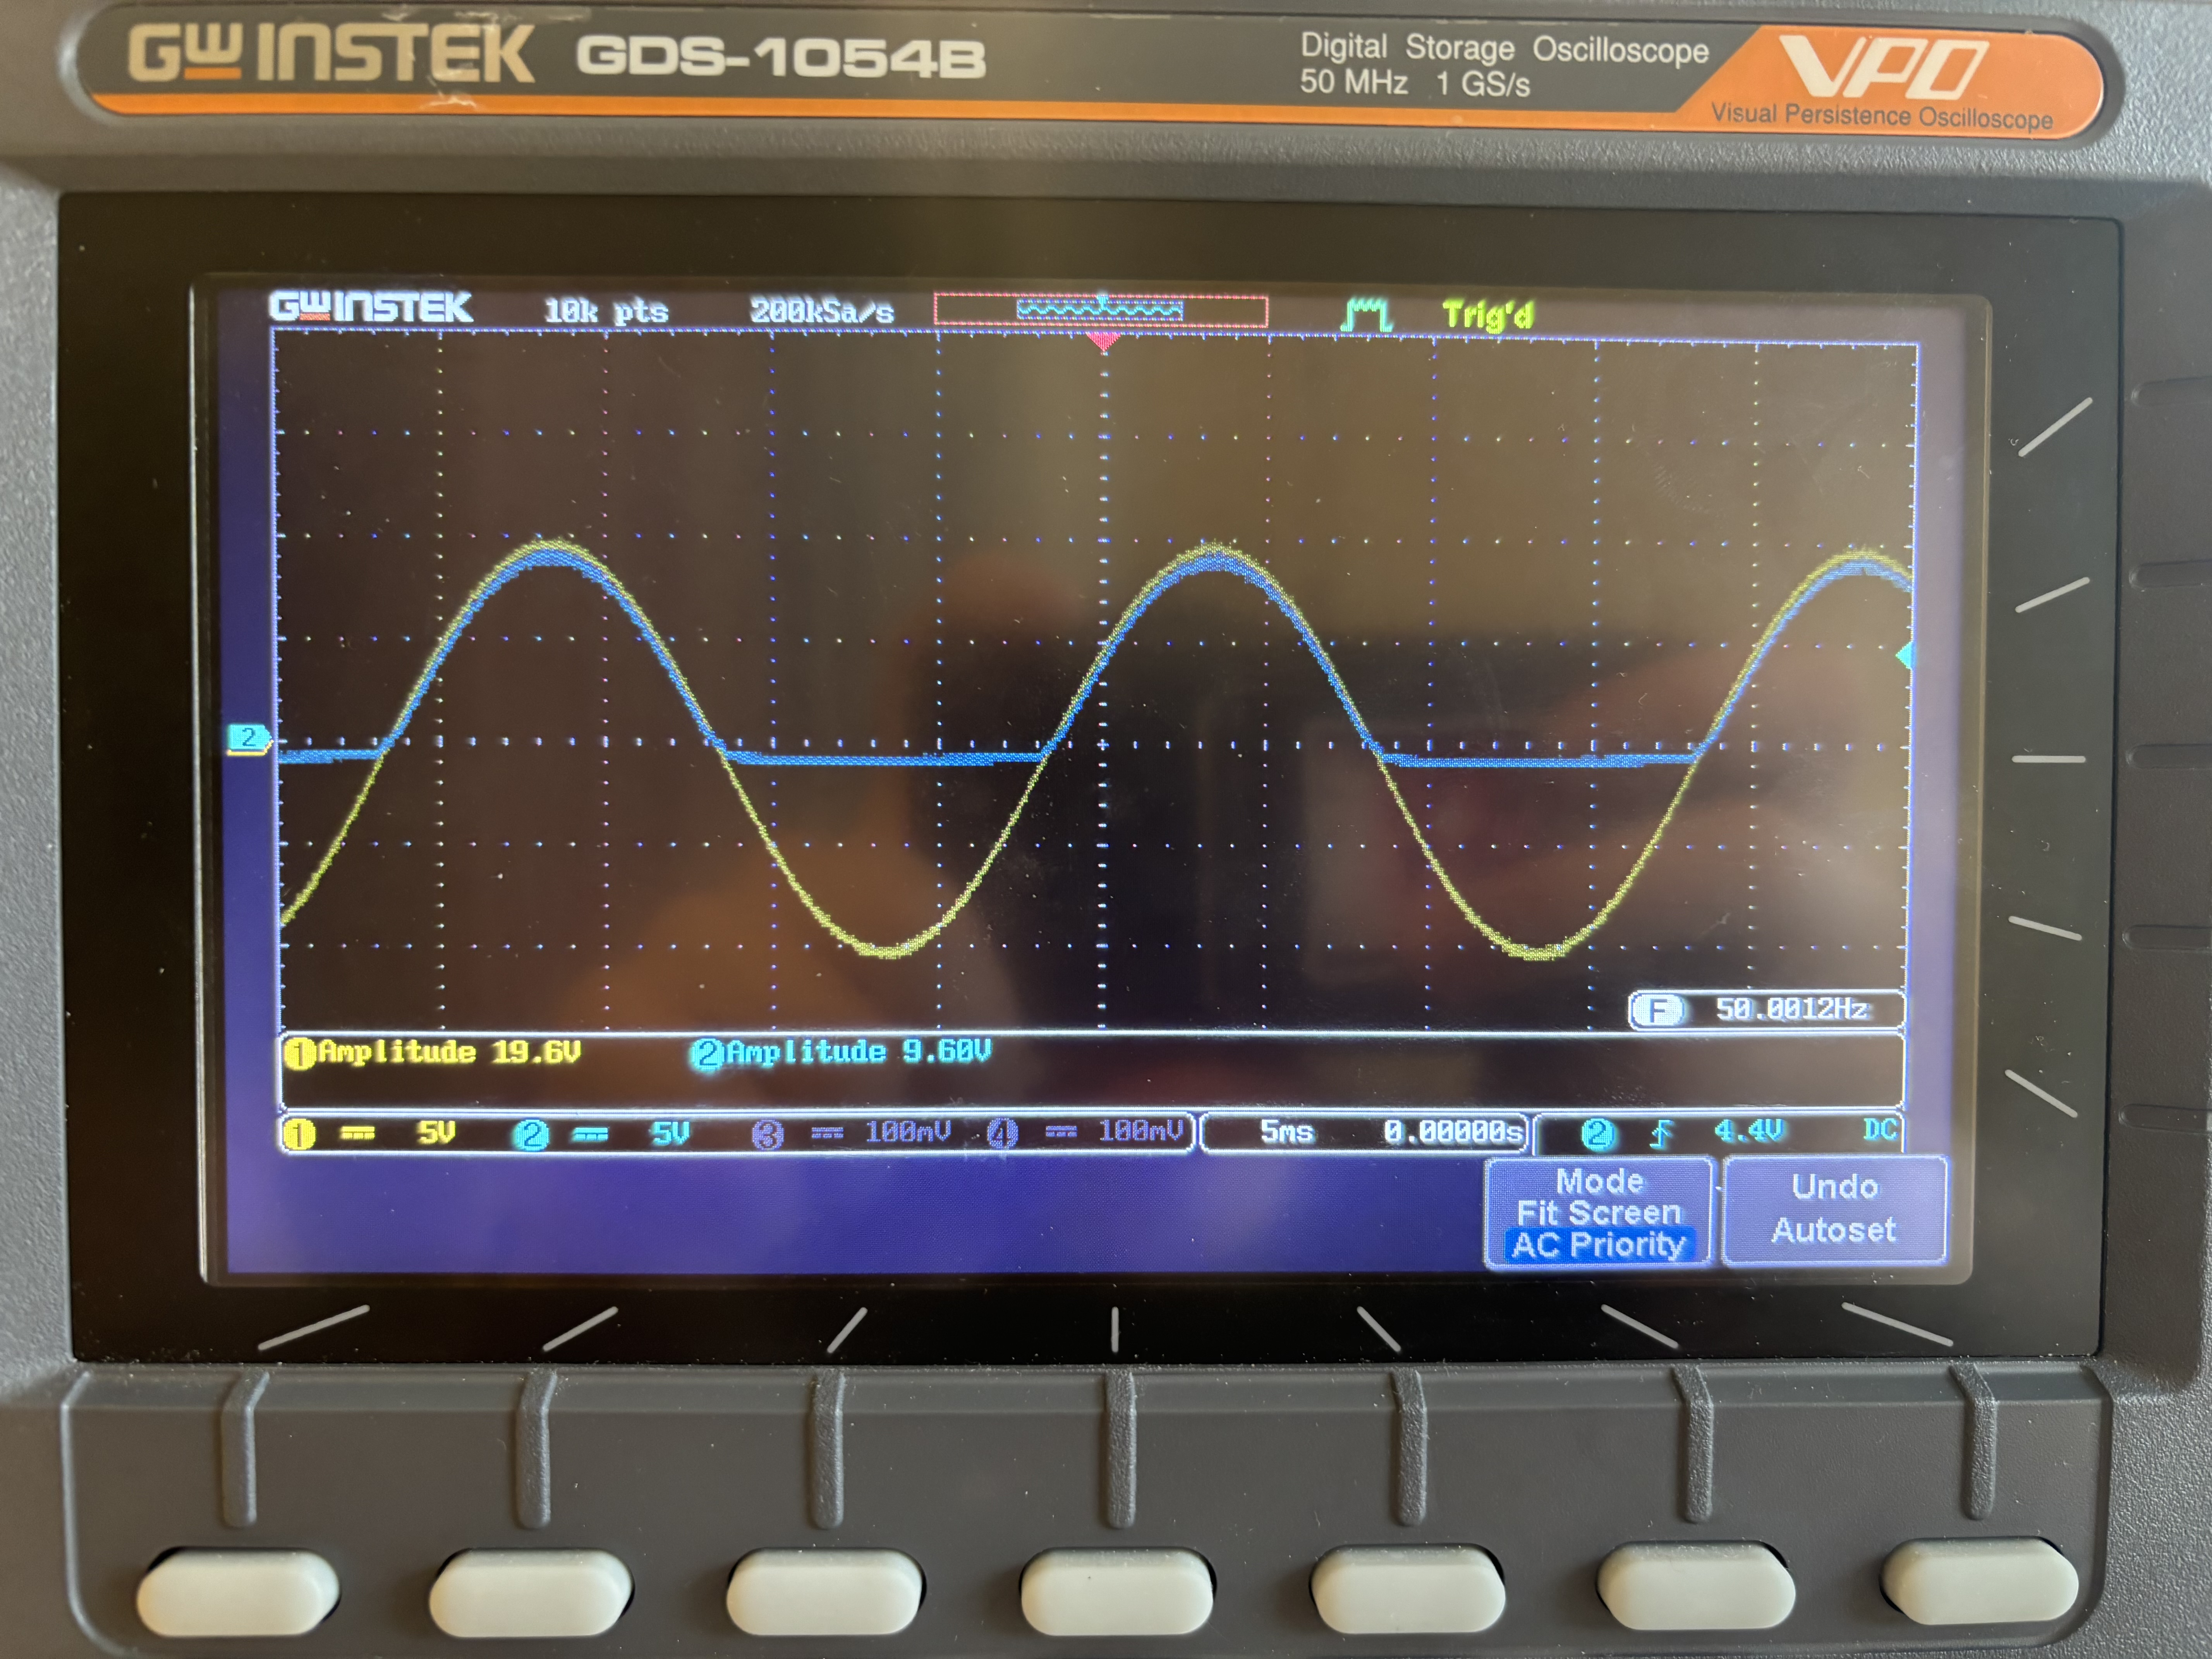
\includegraphics[width=0.85\textwidth]{Media/krets5_ingen_transformator.jpg}
    \caption{Oscilloskopbilde av utgangsspenning i krets 5}\label{fig:krets5_ingen_transformator-oscillskop}
\end{figure}

\vspace{3em}

\begin{figure}[H]
\centering
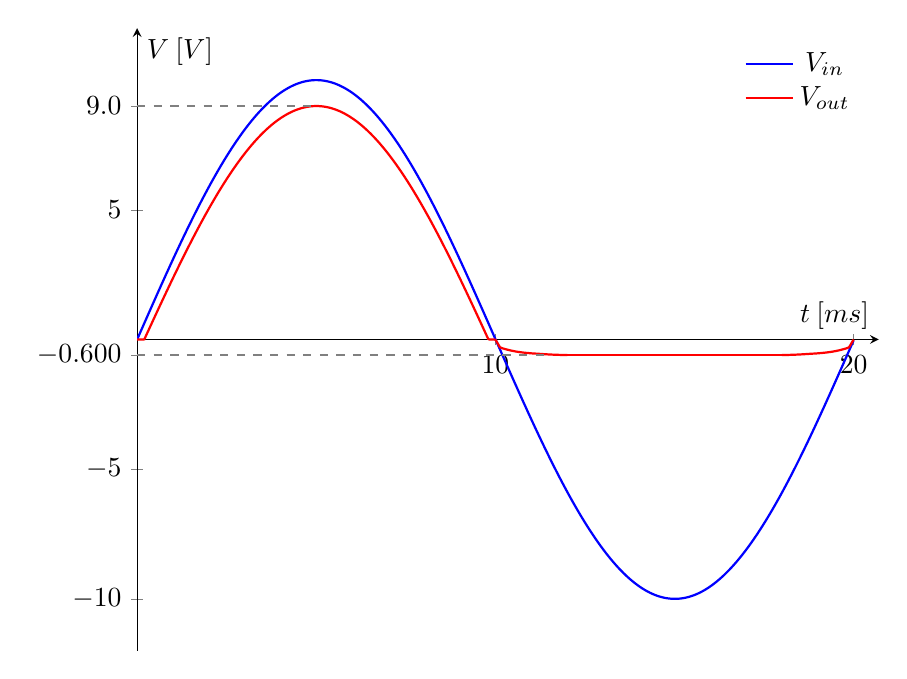
\begin{tikzpicture}
\begin{axis}[
    width=11cm,
    axis lines=middle,
    xlabel={$t\:[ms]$},
    ylabel={$V\:[V]$},
    xmin=0, xmax=6.5,
    ymin=-12, ymax=12,
    samples=300,
    domain=0:6.28,
    ytick={-10,-5,-0.6, 0,5,9},
    yticklabels={$-10$, $-5$, $-0.600$, $0$, $5$, $9.0$},
    xtick={3.14,6.28},
    xticklabels={$10$, $20$},
    legend style={
        at={(0.98,0.98)},
        anchor=north east,
        draw=none,
        fill=none
    }
]

% Inngangsspenning
\addplot[
    blue,
    thick
] {10*sin(deg(x))};
\addlegendentry{$V_{in}$}

\addplot[
    red,
    thick,
    domain=0:3.14
] {max(10*sin(deg(x)) -0.6 - 0.4*sin(deg(x)), 0)};
\addlegendentry{$V_{out}$}

\addplot[
    red,
    thick,
    smooth
] coordinates {
    (3.14, 0.00)
    (3.15, -0.075)
    (3.16, -0.15)
    (3.17, -0.225)
    (3.18, -0.30)
    (3.20, -0.3375)
    (3.23, -0.375)
    (3.27, -0.42)
    (3.32, -0.465)
    (3.38, -0.5025)
    (3.45, -0.5325)
    (3.53, -0.555)
    (3.61, -0.5775)
    (3.69, -0.5925)
    (3.77, -0.60)
};

\addplot[
    red,
    thick
] coordinates {(3.77, -0.60) (5.65, -0.60)};

\addplot[
    red,
    thick,
    smooth
] coordinates {
    (5.65, -0.60)
    (5.69, -0.59625)
    (5.73, -0.5925)
    (5.81, -0.5775)
    (5.89, -0.555)
    (5.97, -0.5325)
    (6.04, -0.5025)
    (6.10, -0.465)
    (6.15, -0.42)
    (6.19, -0.375)
    (6.22, -0.3375)
    (6.24, -0.30)
    (6.25, -0.225)
    (6.26, -0.15)
    (6.27, -0.075)
    (6.28, 0.00)
};

% Klippelinjer
\addplot[dashed, gray] coordinates {(0,-0.6) (3.57,-0.6)};



% Hjelpelinjer
\addplot[
    dashed,
    gray
] coordinates {(0,9) (1.57,9)};

\end{axis}
\end{tikzpicture}
\caption{Måleresultat for krets 5.}\label{fig:resultat_krets5_uten_transformator}
\end{figure}

\clearpage
\noindent
I tillegg måler vi DC-verdien i dette tilfellet, ved å bruke et multimeter i DC-spenningsmåle-modus, som kobles over motstanden i kretsen. Resultatet er i tabellen under.

\begin{table}[H]
\centering
\caption{Resultat for DC-verdier i krets 5.}
\label{tab:krets5_dc_verdi}
\begin{tabular}{lccc}
\toprule
\textbf{Komponent} & \textbf{Teoretisk verdi} & \textbf{Målt verdi} & \textbf{Avvik [\%]} \\
\midrule

% --- Fyll inn rader her ---
% Eksempel:
$V_{DC}$ & $5.04\text{V}$ & $2.54\text{V}$ & 49.6\% \\


% Du kan også lage grupper med tom linje hvis ønskelig

\bottomrule
\end{tabular}
\end{table}

\paragraph{Kommentar til resultater. } Ekstremalpunktene i grafen er målt med cursors på oscilloskopet. Grafen for utgangsspenningen er ikke som forventet. Den oppfører seg som en enveis likeretter, hvor også den negative halvbølgen klippes ved $-600\mathrm{mV}$. Dette skyldes jordingsfeil i kretsen. Ved å benytte en transformator som inngangsspenning, vil vi kunne måle resultatet for en toveis likeretter uten jordingsfeil.

\paragraph{Bruk av transformator. } Fremgangsmåten for å koble opp krets 5 med transformator er i utgangspunktet lik som uten transformator. Forskjellen er at signalgeneratoren ikke benyttes. I stedet kobler vi en transformator til strømnettet, og bruker den som inngangsspenning for kretsen. For å måle på kretsen må vi passe på jordingsforholdene. Vi kan ikke måle inngangsspenningen samtidig som utgangsspenningen, da dette vil skape en jordingsfeil. I dette forsøket er inngangsspenning og utgangsspenning målt hver for seg og tegnet i samme graf.

\vspace{2em}

\begin{figure}[H]
    \centering
    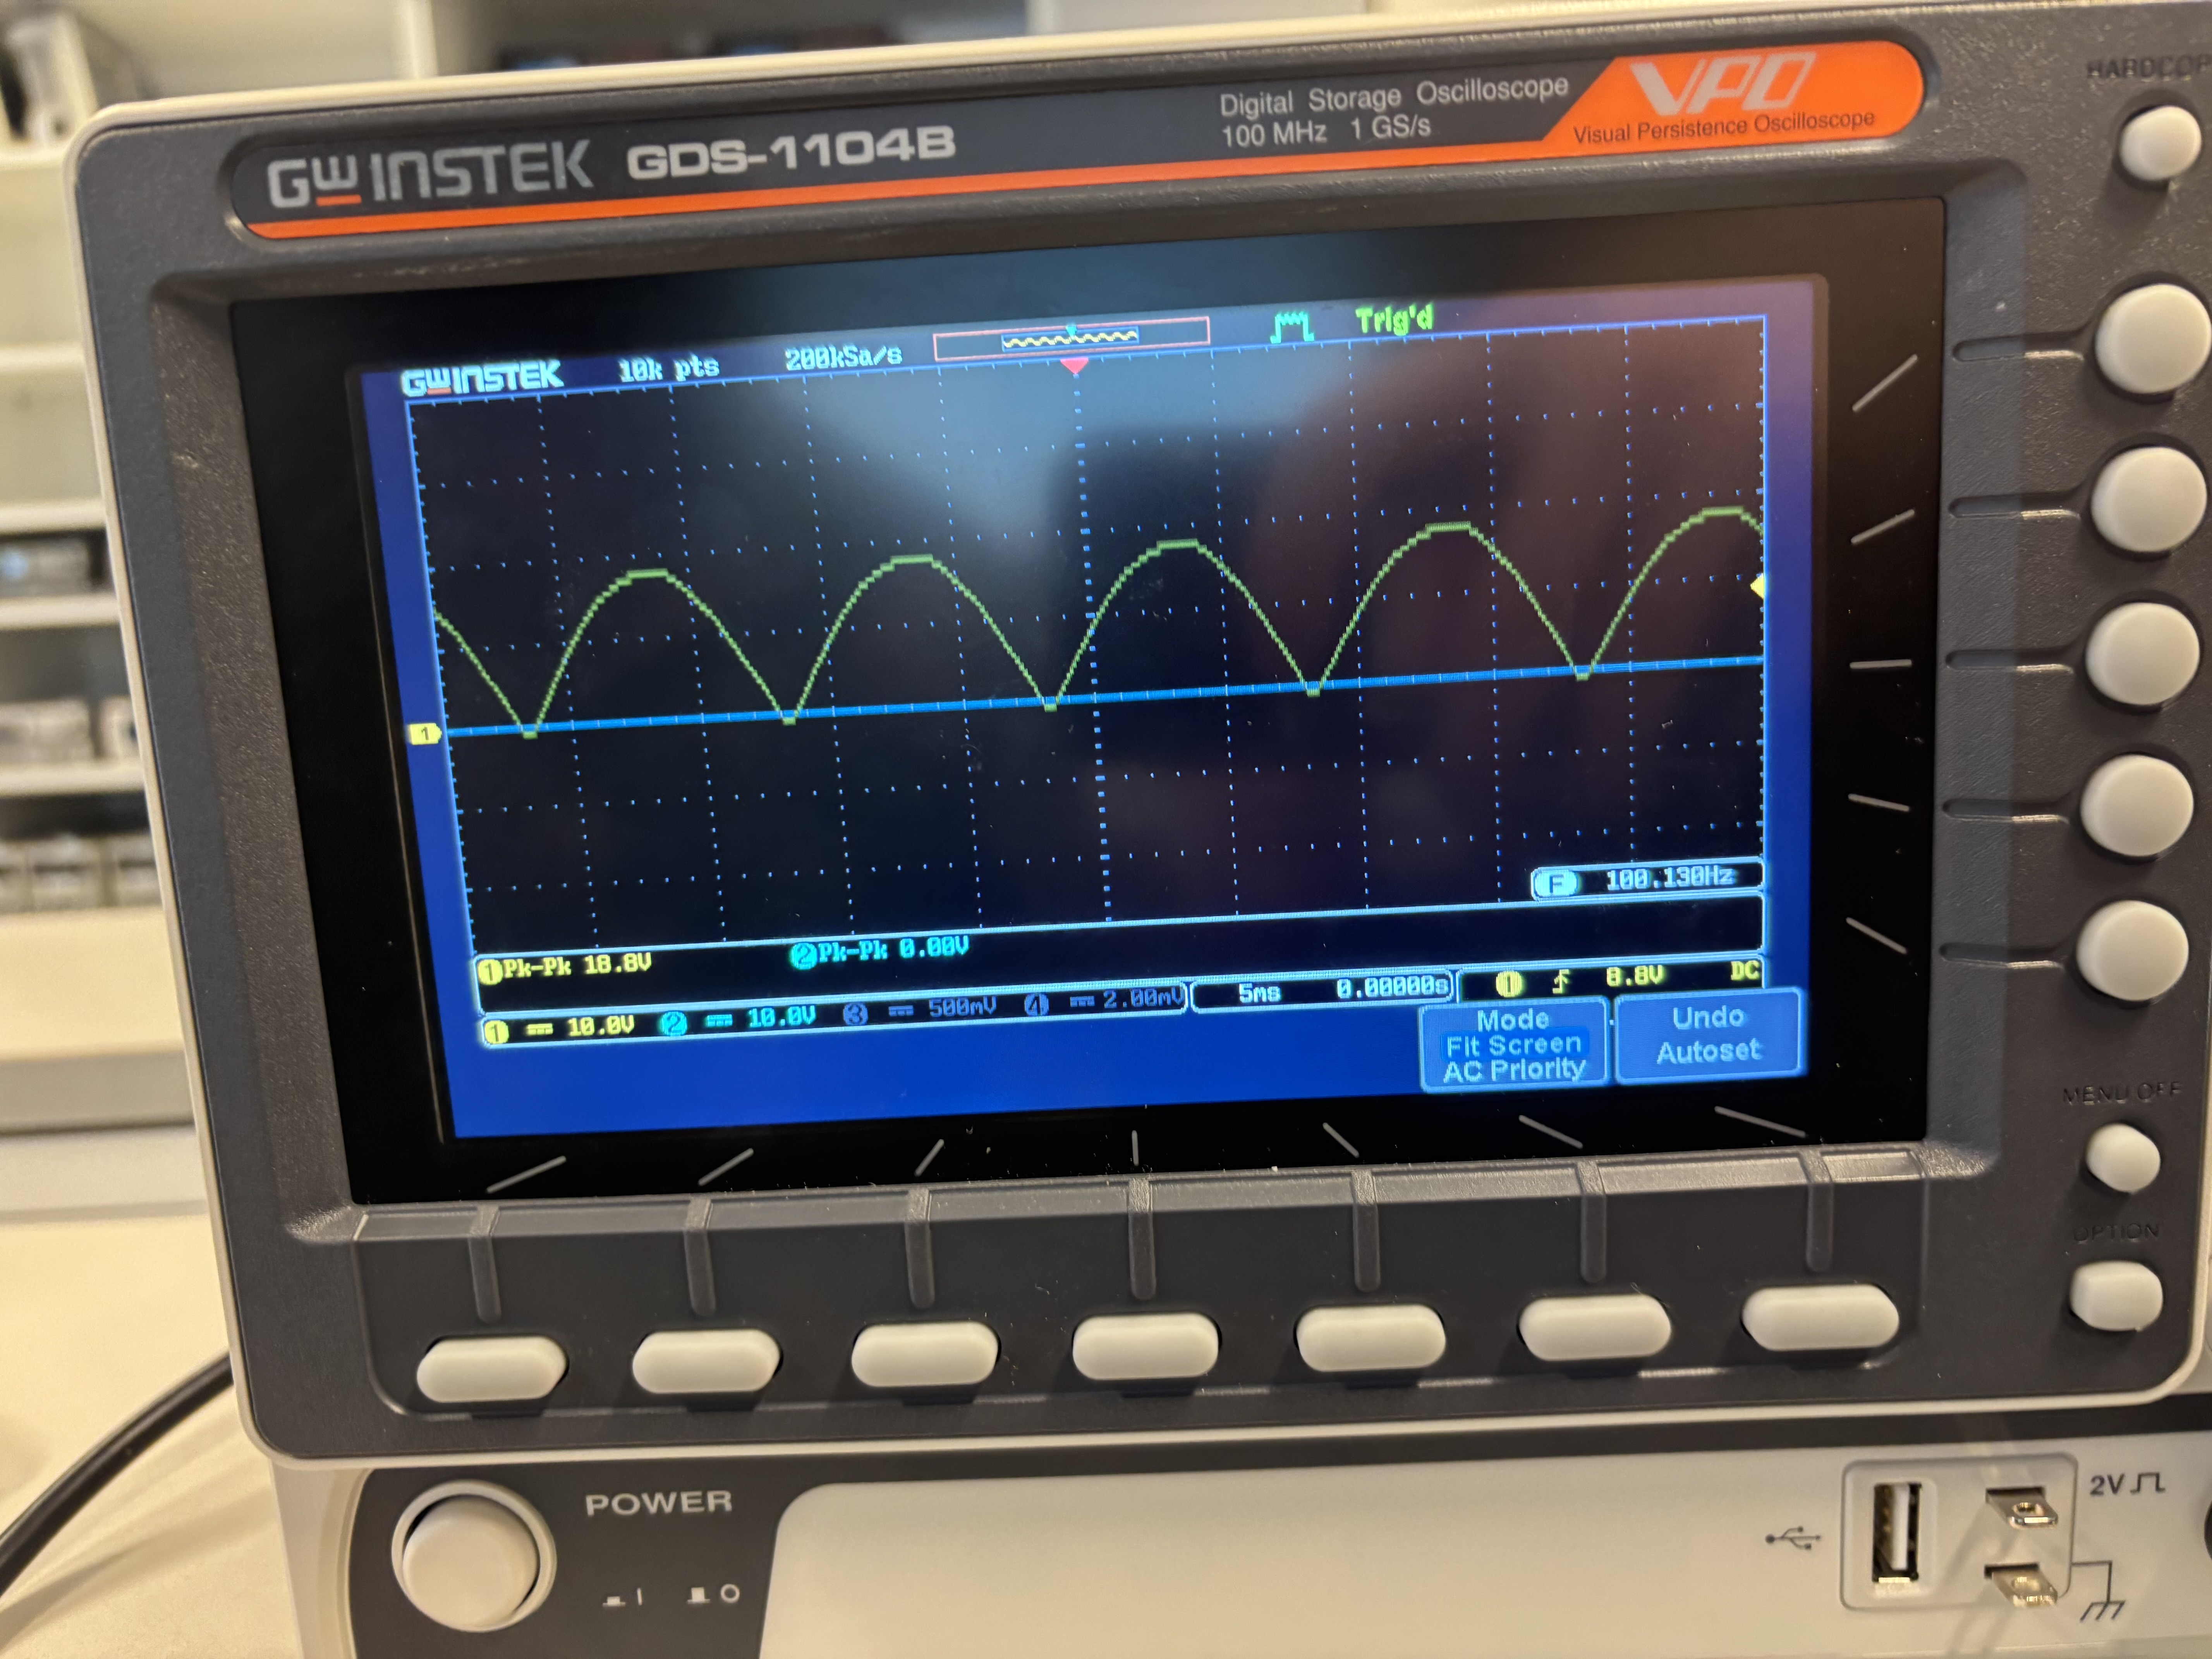
\includegraphics[width=0.85\textwidth]{Media/krets5_med_transformator.jpg}
    \caption{Oscilloskopbilde av utgangsspenning i krets 5 med bruk av transformator}\label{fig:krets5_med_transformator-oscillskop}
\end{figure}


\begin{figure}[H]
\centering
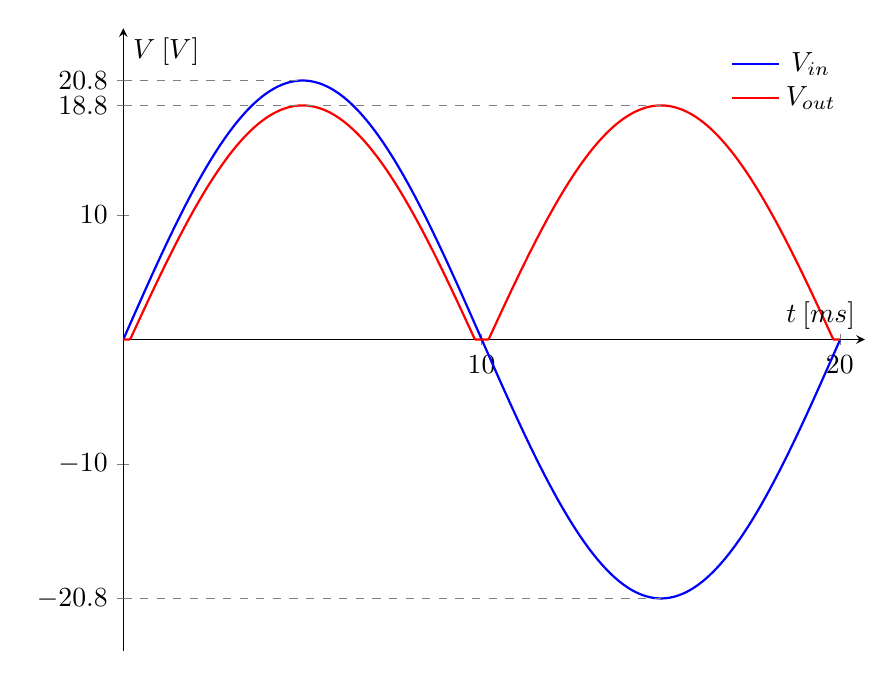
\begin{tikzpicture}
\begin{axis}[
    width=11cm,
    axis lines=middle,
    xlabel={$t\:[ms]$},
    ylabel={$V\:[V]$},
    xmin=0, xmax=6.5,
    ymin=-25, ymax=25,
    samples=300,
    domain=0:6.28,
    ytick={-20.8,-10, 0,10,18.8, 20.8},
    yticklabels={$-20.8$, $-10$, $0$, $10$, $18.8$, $20.8$},
    xtick={3.14,6.28},
    xticklabels={$10$, $20$},
    legend style={
        at={(0.98,0.98)},
        anchor=north east,
        draw=none,
        fill=none
    }
]

% Inngangsspenning
\addplot[
    blue,
    thick
] {20.8*sin(deg(x))};
\addlegendentry{$V_{in}$}

\addplot[
    red,
    thick,
    domain=0:3.14
] {max(20.8*sin(deg(x)) -1.2 - 0.8*sin(deg(x)), 0)};
\addlegendentry{$V_{out}$}

\addplot[
    red,
    thick,
    domain=3.14:6.28
] {max(- 20.8*sin(deg(x)) -1.2 + 0.8*sin(deg(x)), 0)};

% Hjelpelinjer
\addplot[
    dashed,
    gray
] coordinates {(0,18.8) (4.71,18.8)};

\addplot[
    dashed,
    gray
] coordinates {(0,20.8) (1.57,20.8)};

\addplot[
    dashed,
    gray
] coordinates {(0,-20.8) (4.71,-20.8)};

\end{axis}
\end{tikzpicture}
\caption{Måleresultat for krets 5 ved bruk av transformator som inngangsspenning.}\label{fig:resultat_krets5_med_transformator}
\end{figure}

\begin{table}[H]
\centering
\caption{Resultat for DC-verdier i krets 5 ved bruk av transformator som inngangsspenning.}
\label{tab:krets5_dc_verdi_transformator}
\begin{tabular}{lc}
\toprule
\textbf{Komponent}& \textbf{Målt verdi} \\
\midrule

% --- Fyll inn rader her ---
% Eksempel:
$V_{DC}$ & $11.17\text{V}$ \\


% Du kan også lage grupper med tom linje hvis ønskelig

\bottomrule
\end{tabular}
\end{table}

\paragraph{Kommentar til resultater ved bruk av transformator. } Resultatene er mer som forventet, da jordingsfeilene er eliminert. Vi kan også merke oss av et endret inngangssignal. Frekvensen er den samme på $50\text{Hz}$, men amplituden er nå målt $20.8\mathrm{V}$ i stedet for $10\mathrm{V}$. Verdiene kan ikke sammenliknes direkte med teoriseksjonen for denne kretsen, på grunn av et endret inngangsspenning. Uansett, kan vi se at den karakteristiske toveis likeretterkurven er som forventet, med et spenningstap på $2.0\mathrm{V}$ over to dioder. DC-verdien er også målt til $11.17\mathrm{V}$, som er forventet høyere enn det teoretiske med dens høyere inngangsspenning. Resultatene her er uten store avvik og er forventet.

\subsection{Krets 6 -- toveis likeretter med kondensator}

Vi benytter transformator som inngangsspenning. Oppkoblingen utenom signalgeneratoren, er lik som i kretsen presentert i figur~\ref{fig:krets6}. Vi bruker en motstand på $1\mathrm{k\Omega}$ i serie med fire dioder som er koblet i en brokonfigurasjon, og en kondensator. Vi skal foreta målinger i to tilfeller: først med en kondensator på $100\mu\text{F}$, og deretter med en kondensator på $10\mu\text{F}$. Resultatene er i figurene under.


\begin{figure}[H]
\centering

\begin{subfigure}{0.48\textwidth}
    \centering
    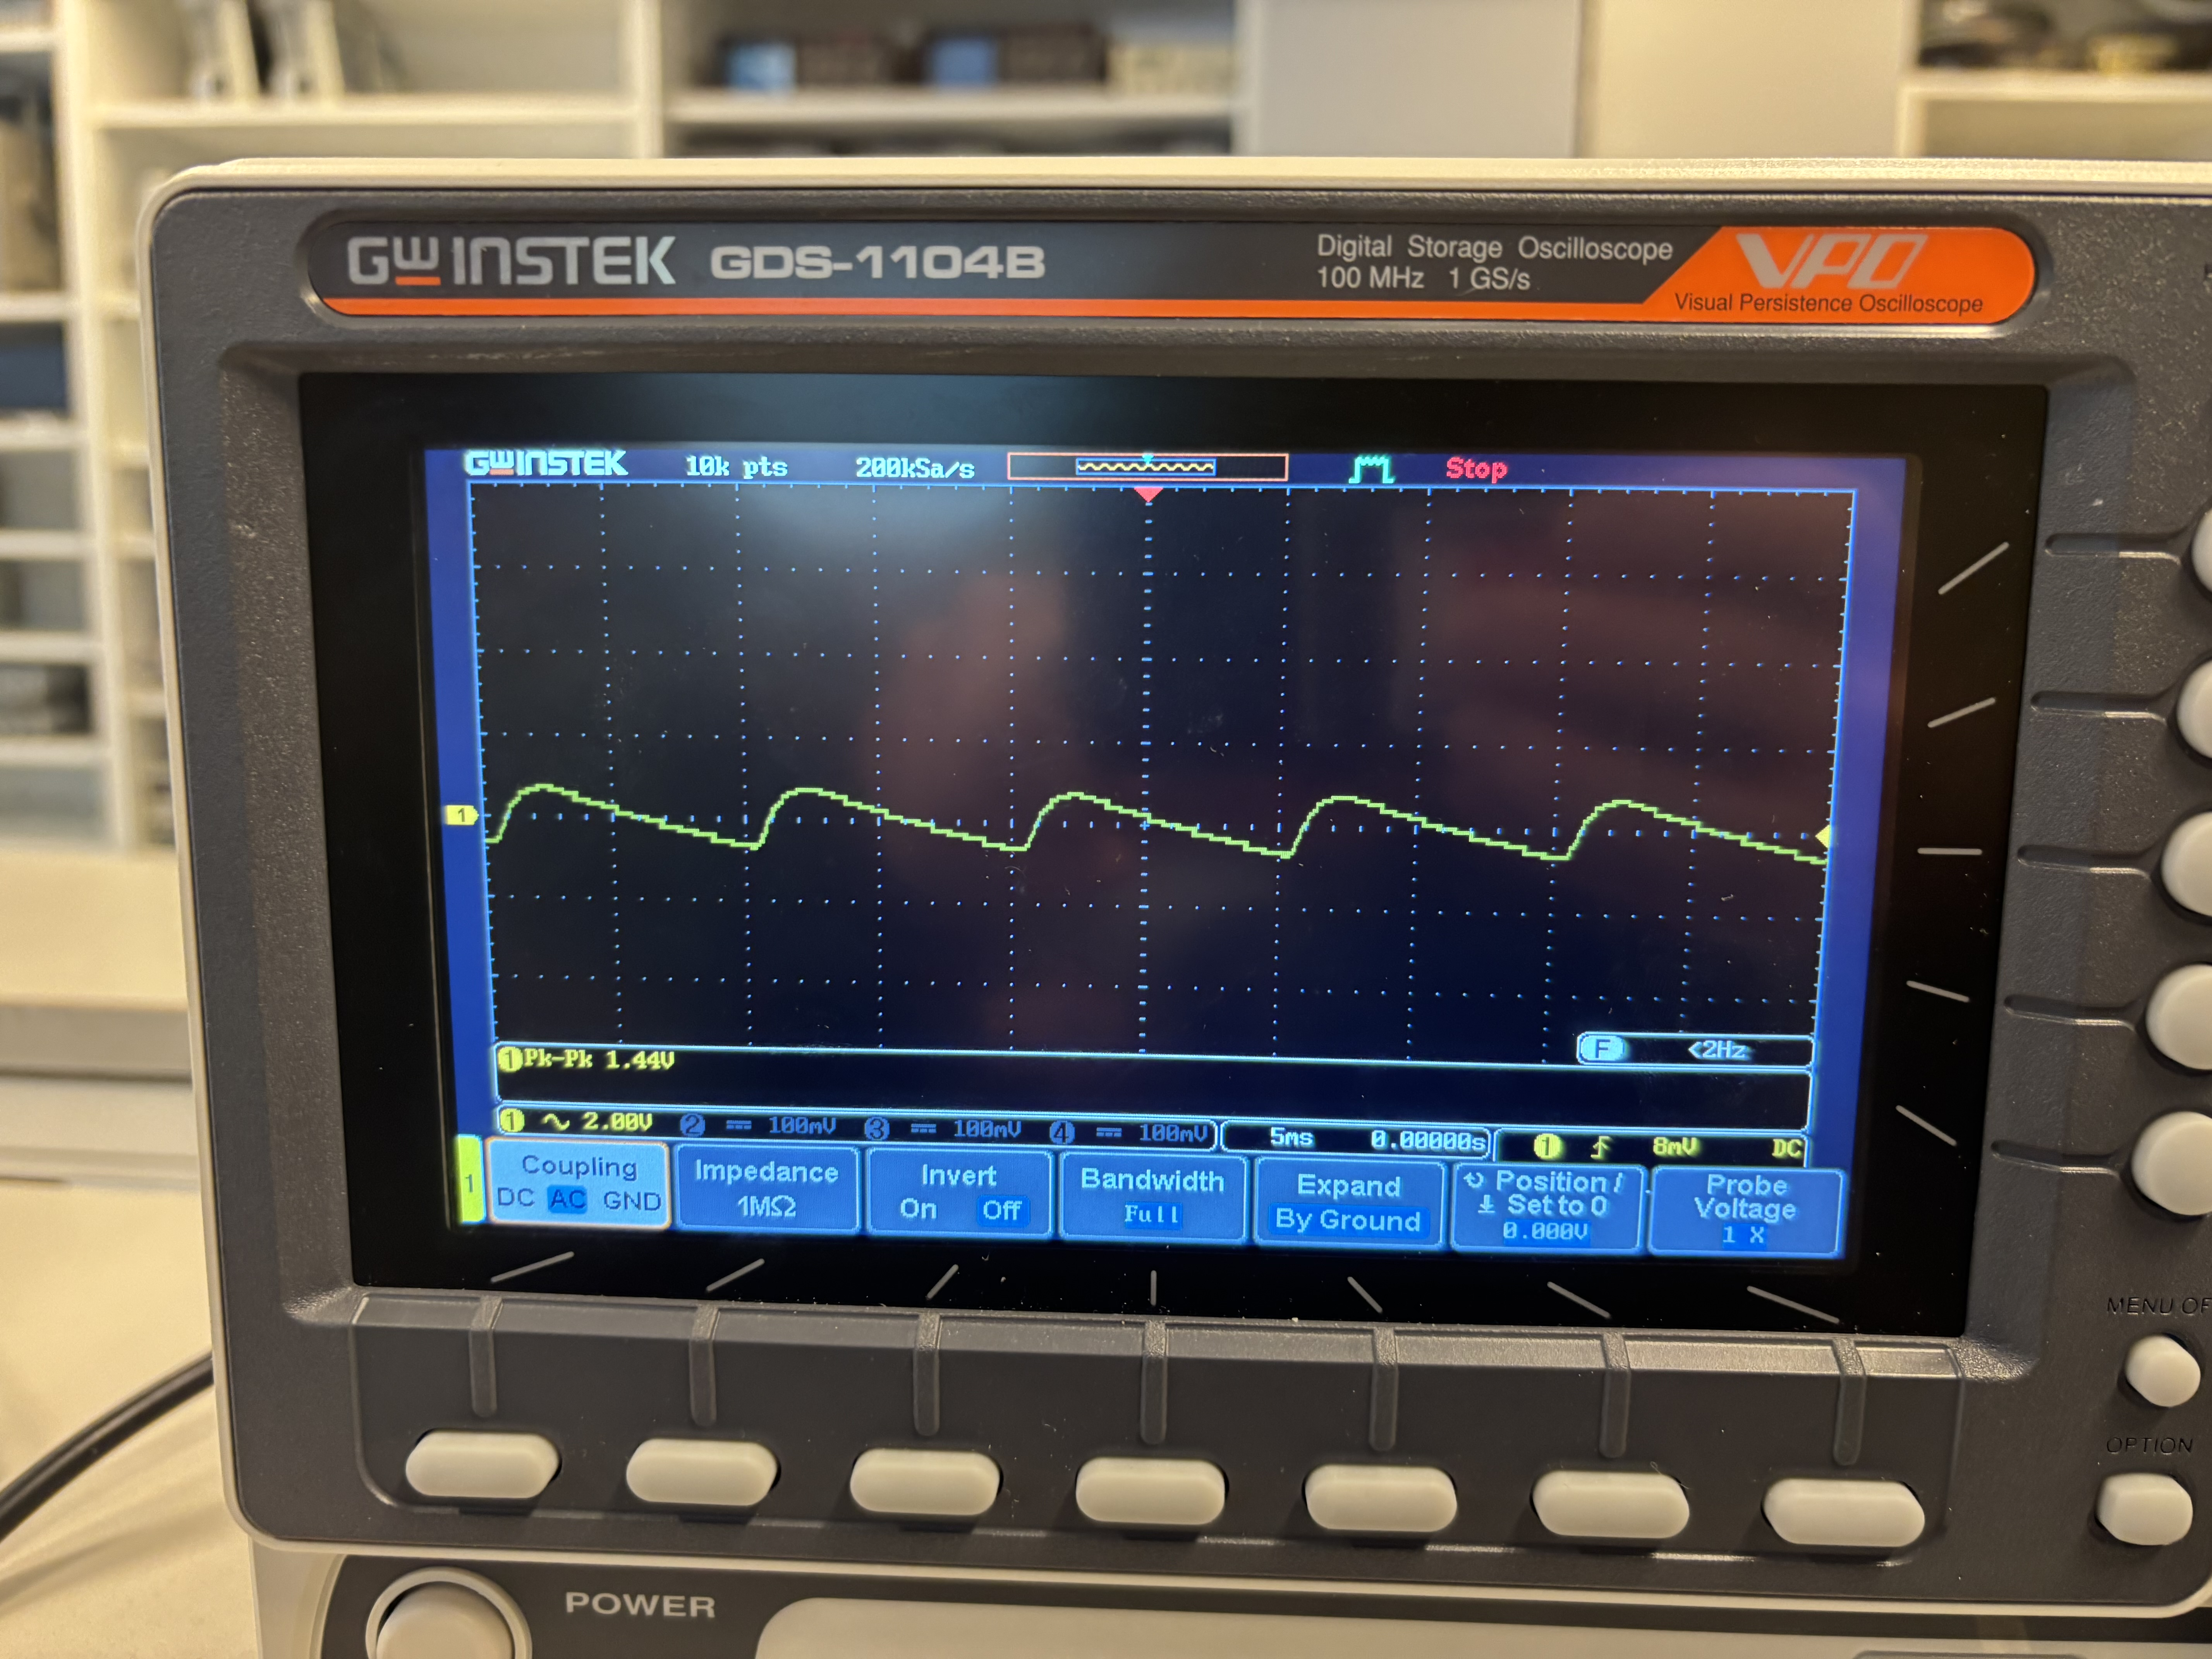
\includegraphics[width=\linewidth]{Media/krets6_100.jpg}
    \caption{Kapasitans på $100\mu \text{F}$}
    \label{fig:krets6_100}
\end{subfigure}
\hfill
\begin{subfigure}{0.48\textwidth}
    \centering
    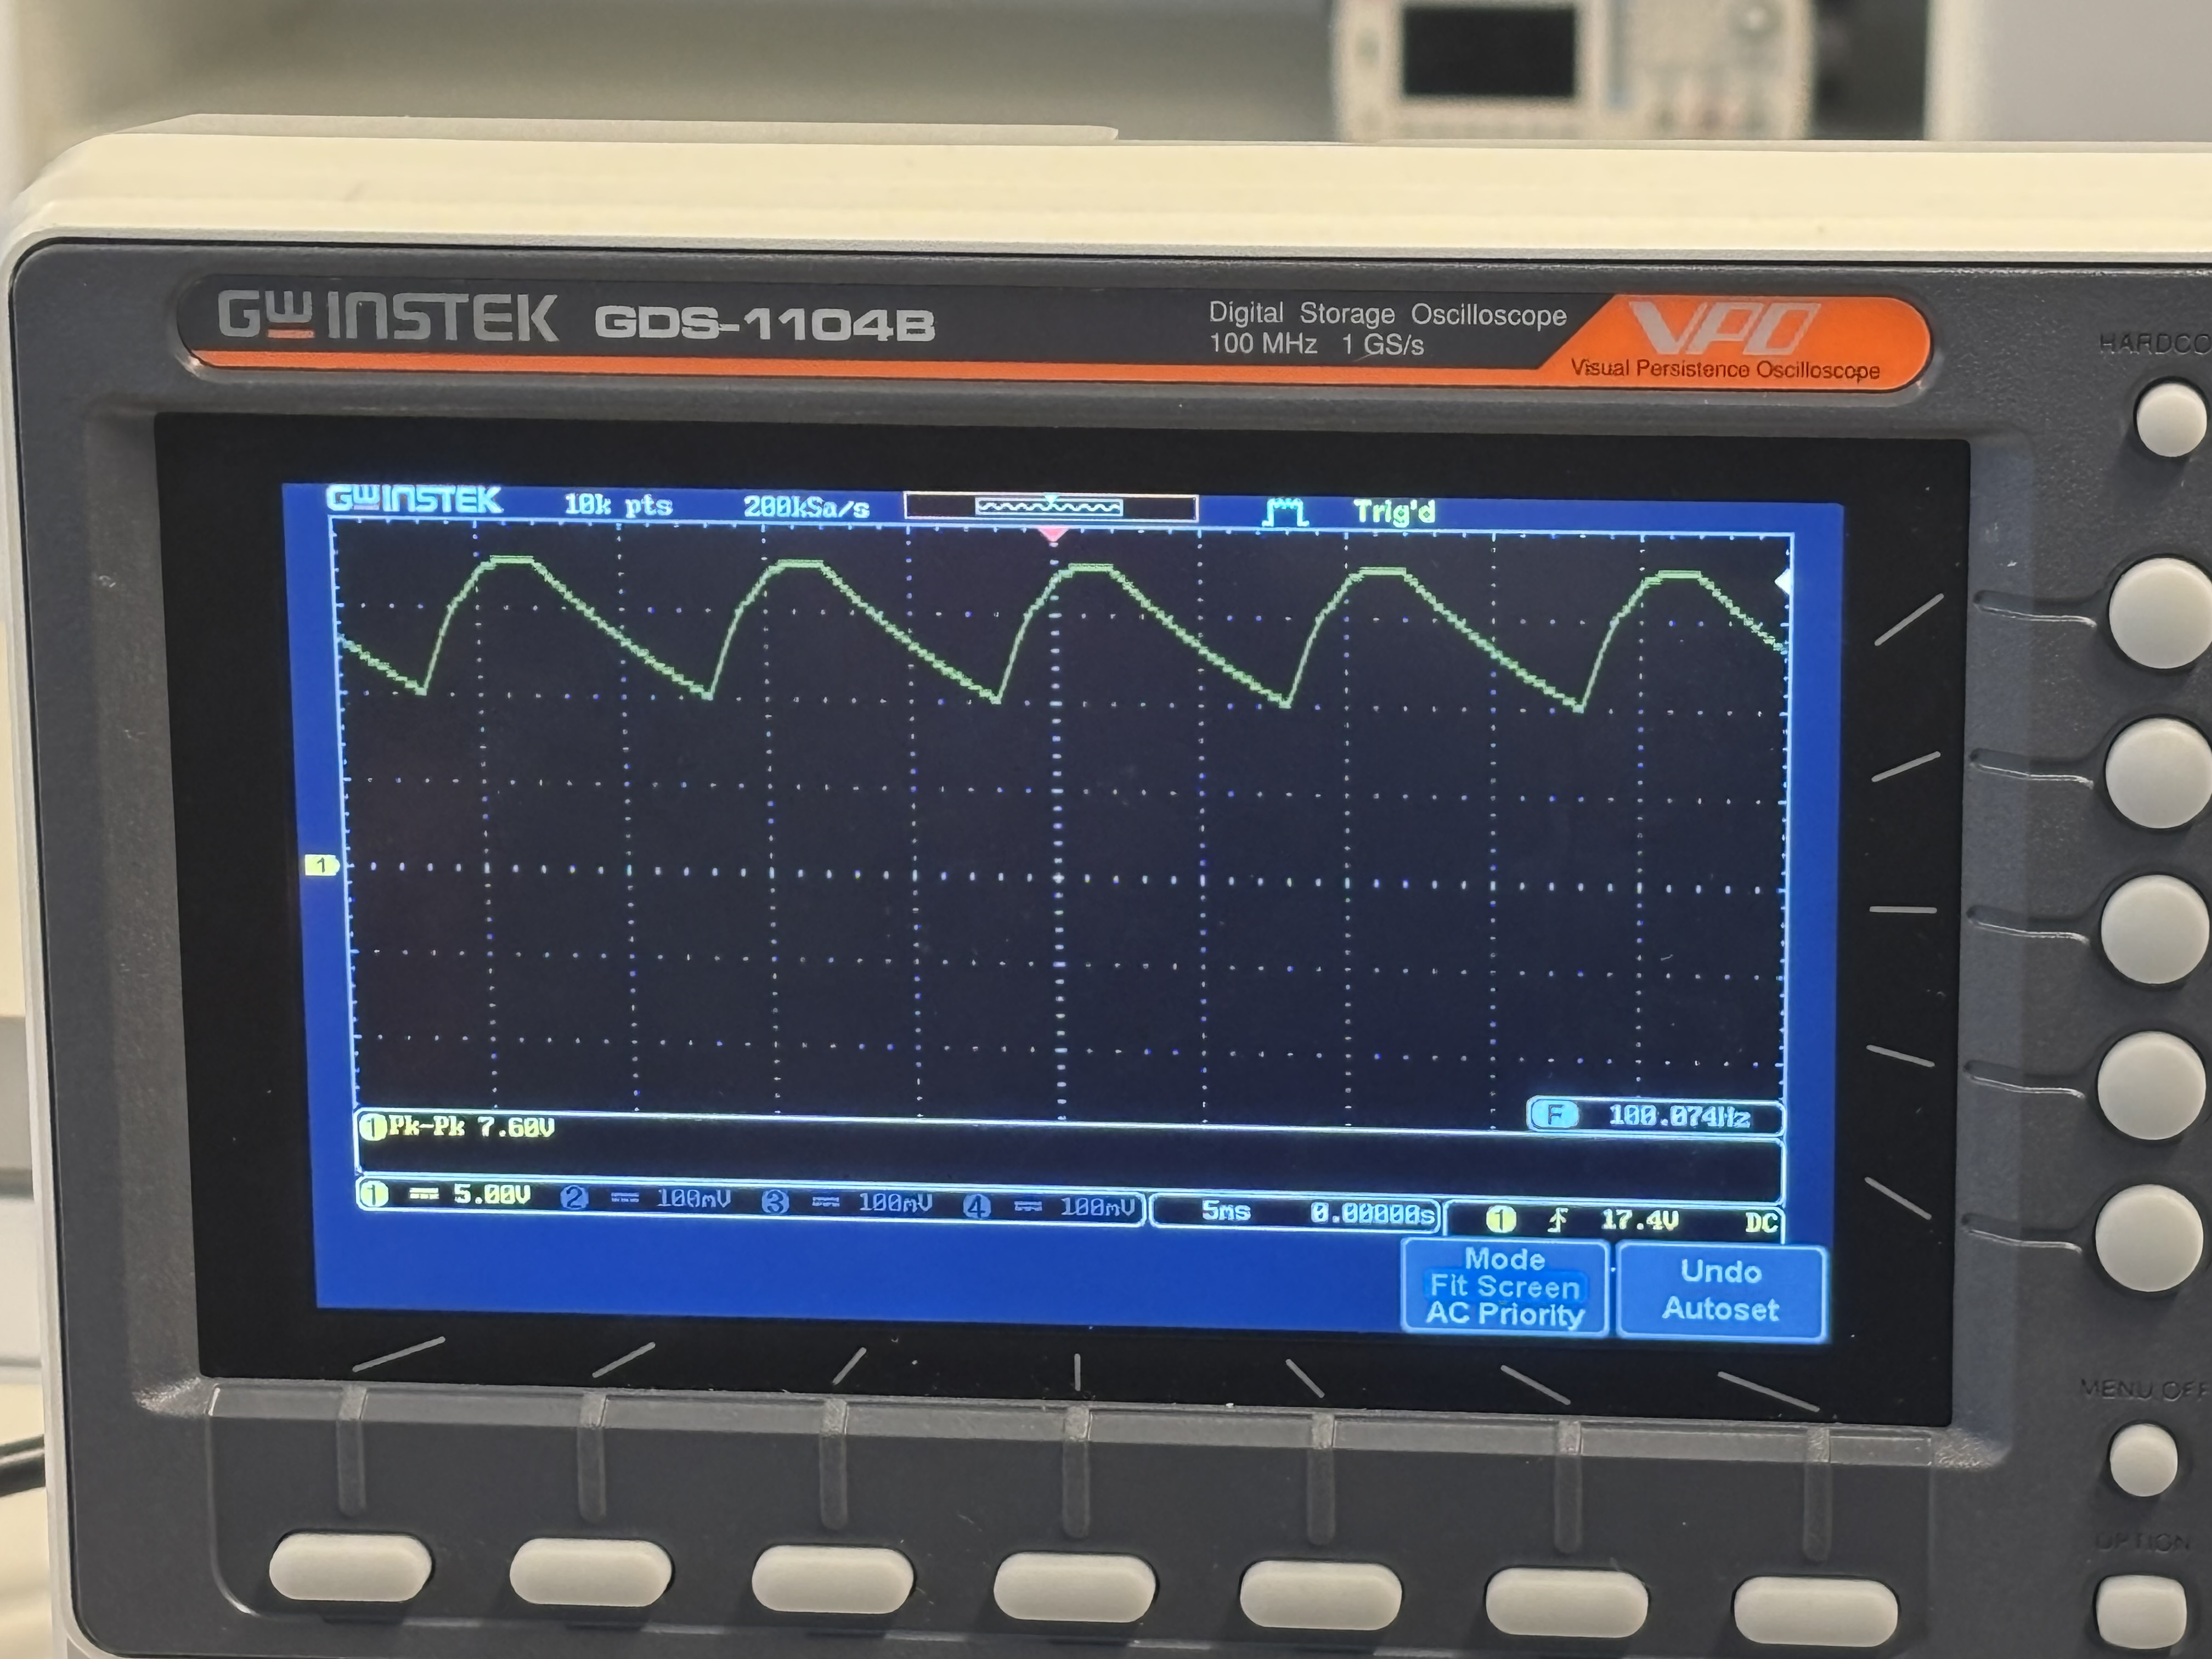
\includegraphics[width=\linewidth]{Media/krets6_10.jpg}
    \caption{Kapasitans på $10\mu \text{F}$}
    \label{fig:krets6_10}
\end{subfigure}

\caption{Oscilloskopbilder av utgangsspenning i krets 6}
\label{fig:krets6_oscillo}
\end{figure}

\begin{figure}[H]
\centering
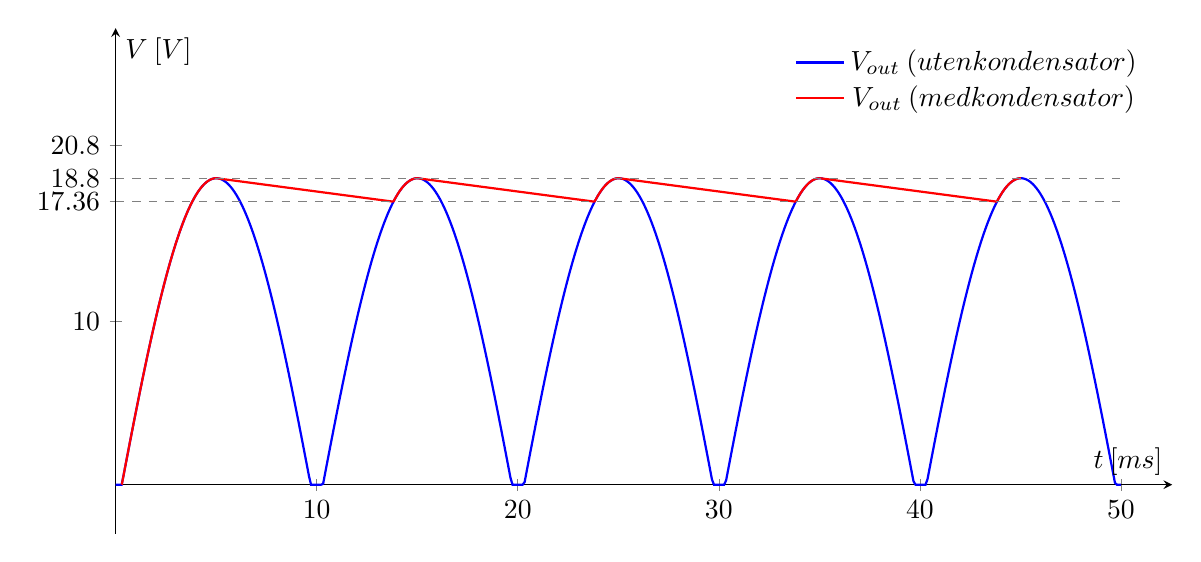
\begin{tikzpicture}
\begin{axis}[
    width=15cm,
    height=8cm,
    axis lines=middle,
    xlabel={$t \: [ms]$},
    ylabel={$V \: [V]$},
    xmin=0, xmax=16.5,
    ymin=-3, ymax=28,
    samples=500,
    domain=0:15.7,
    ytick={0,10,17.36,18.8,20.8},
    yticklabels={$0$, $10$, $17.36$, $18.8$, $20.8$},
    xtick={3.14,6.28,9.42,12.56,15.7},
    xticklabels={$10$, $20$, $30$, $40$, $50$},
    legend style={
        at={(0.98,0.98)},
        anchor=north east,
        draw=none,
        fill=none
    }
]

% Utgang uten kondensator
\addplot[
    blue,
    thick
] {max(0, abs(20.8 * sin(deg(x))) - 2)};
\addlegendentry{$V_{out} \: \text{(uten kondensator)}$}

% Utgang med kondensator: første opplading
\addplot[
    red,
    thick,
    domain=0.0963:pi/2
] {abs(20.8 * sin(deg(x))) - 2};
\addlegendentry{$V_{out} \: \text{(med kondensator)}$}

% Periode 1: utlading + ny opplading
\addplot[red, thick] coordinates {
    (1.571, 18.8)
    (4.338, 17.36)
};
\addplot[
    red,
    thick,
    domain=4.338:3*pi/2
] {abs(20.8 * sin(deg(x))) - 2};

% Periode 2
\addplot[red, thick] coordinates {
    (4.712, 18.8)
    (7.480, 17.36)
};
\addplot[
    red,
    thick,
    domain=7.480:5*pi/2
] {abs(20.8 * sin(deg(x))) - 2};

% Periode 3
\addplot[red, thick] coordinates {
    (7.854, 18.8)
    (10.622, 17.36)
};
\addplot[
    red,
    thick,
    domain=10.622:7*pi/2
] {abs(20.8 * sin(deg(x))) - 2};

% Periode 4
\addplot[red, thick] coordinates {
    (10.996, 18.8)
    (13.763, 17.36)
};
\addplot[
    red,
    thick,
    domain=13.763:9*pi/2
] {abs(20.8 * sin(deg(x))) - 2};

\addplot[
    dashed,
    gray
] coordinates {(0,17.36) (15.7,17.36)};

\addplot[
    dashed,
    gray
] coordinates {(0,18.8) (15.7,18.8)};

\end{axis}
\end{tikzpicture}
\caption{Resultat for krets 6, kapasitansen er $100\mu\text{F}$.}
\label{fig:rectifier_with_capacitor_in_out_100}
\end{figure}


\begin{figure}[H]
\centering
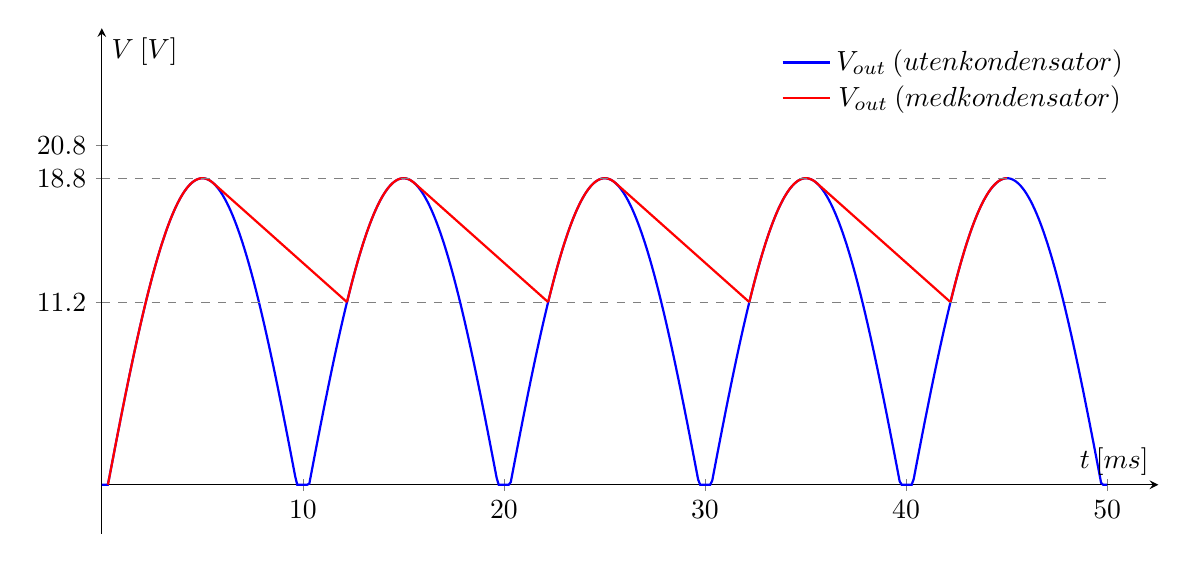
\begin{tikzpicture}
\begin{axis}[
    width=15cm,
    height=8cm,
    axis lines=middle,
    xlabel={$t \: [ms]$},
    ylabel={$V \: [V]$},
    xmin=0, xmax=16.5,
    ymin=-3, ymax=28,
    samples=500,
    domain=0:15.7,
    ytick={0,11.2,18.8,20.8},
    yticklabels={$0$,$11.2$, $18.8$, $20.8$},
    xtick={3.14,6.28,9.42,12.56,15.7},
    xticklabels={$10$, $20$, $30$, $40$, $50$},
    legend style={
        at={(0.98,0.98)},
        anchor=north east,
        draw=none,
        fill=none
    }
]

% Definerer likerettet signal med 2 V diodetap
\addplot[
    blue,
    thick
] {max(0, abs(20.8*sin(deg(x))) - 2)};
\addlegendentry{$V_{out}\:\text{(uten kondensator)}$}

% Rød: med kondensator
\addplot[
    red,
    thick,
    domain=0.0963:1.740
] {abs(20.8*sin(deg(x))) - 2};
\addlegendentry{$V_{out}\:\text{(med kondensator)}$}

% Første lineære utlading
\addplot[
    red,
    thick
] coordinates {
    (1.740, 18.504)
    (3.829, 11.2)
};

% Neste sinusoppgang
\addplot[
    red,
    thick,
    domain=3.829:3*pi/2
] {abs(20.8*sin(deg(x))) - 2};

% Periode 2
\addplot[red, thick, domain=3*pi/2:4.882] {abs(20.8*sin(deg(x))) - 2};
\addplot[red, thick] coordinates {
    (4.882, 18.504)
    (6.971, 11.2)
};
\addplot[red, thick, domain=6.971:5*pi/2] {abs(20.8*sin(deg(x))) - 2};

% Periode 3
\addplot[red, thick, domain=5*pi/2:8.023] {abs(20.8*sin(deg(x))) - 2};
\addplot[red, thick] coordinates {
    (8.023, 18.504)
    (10.112, 11.2)
};
\addplot[red, thick, domain=10.112:7*pi/2] {abs(20.8*sin(deg(x))) - 2};

% Periode 4
\addplot[red, thick, domain=7*pi/2:11.165] {abs(20.8*sin(deg(x))) - 2};
\addplot[red, thick] coordinates {
    (11.165, 18.504)
    (13.254, 11.2)
};
\addplot[red, thick, domain=13.254:9*pi/2] {abs(20.8*sin(deg(x))) - 2};

% Hjelpelinje
\addplot[
    dashed,
    gray
] coordinates {(0,11.2) (15.7,11.2)};

\addplot[
    dashed,
    gray
] coordinates {(0,18.8) (15.7,18.8)};

\end{axis}
\end{tikzpicture}
\caption{Resultat for krets 6, kapasitansen er $10\mu\text{F}$.}
\label{fig:rectifier_with_capacitor_in_out_10}
\end{figure}

\begin{table}[H]
\centering
\caption{Resultater for DC-verdier i krets 6.}
\label{tab:krets6_dc_verdi_transformator}
\begin{tabular}{lc}
\toprule
\textbf{Komponent} & \textbf{Målt verdi} \\
\midrule

% --- Fyll inn rader her ---
% Eksempel:
$V_{DC} \: \left(100\mu\text{F}\right)$ & $17.16\text{V}$ \\
$V_{DC} \: \left(10\mu\text{F}\right)$ & $14.57\text{V}$ \\


% Du kan også lage grupper med tom linje hvis ønskelig

\bottomrule
\end{tabular}
\end{table}



\paragraph{Kommentar til resultater. } Resultatene er som forventet. Vi kan tydelig se at ved høyere kapasitans, så er ripplet mindre og DC-verdien høyere. Ripple i hver graf er forskjellen mellom toppunkt og bunnpunkt for kondensatorkurven (mellom stiplet grå linjer). For $100\mu\text{F}$ er ripplet på $1.44\mathrm{V}$, og for $10\mu\text{F}$ er ripplet på $7.6\mathrm{V}$. Grafene og teoretiske verdier samsvarer med hverandre. Resultatene er uten store avvik og er som forventet.

